%definira klasu dokumenta 
\documentclass[12pt]{report} 

%prostor izmedu naredbi \documentclass i \begin{document} se zove uvod. U njemu se nalaze naredbe koje se odnose na cijeli dokument

%osnovni LaTex ne može riješiti sve probleme, pa se koriste različiti paketi koji olakšavaju izradu željenog dokumenta
\usepackage[croatian]{babel} 
\usepackage{amssymb}
\usepackage{amsmath}
\usepackage{txfonts}
\usepackage{mathdots}
\usepackage{titlesec}
\usepackage{array}
\usepackage{lastpage}
\usepackage{etoolbox}
\usepackage{tabularray}
\usepackage{color, colortbl}
\usepackage{adjustbox}
\usepackage{geometry}
\usepackage[classicReIm]{kpfonts}
\usepackage{hyperref}
\usepackage{fancyhdr}

\usepackage{float}
\usepackage{setspace}
\restylefloat{table}


\patchcmd{\chapter}{\thispagestyle{plain}}{\thispagestyle{fancy}}{}{} %redefiniranje stila stranice u paketu fancyhdr

%oblik naslova poglavlja
\titleformat{\chapter}{\normalfont\huge\bfseries}{\thechapter.}{20pt}{\Huge}
\titlespacing{\chapter}{0pt}{0pt}{40pt}


\linespread{1.3} %razmak između redaka

\geometry{a4paper, left=1in, top=1in,}  %oblik stranice

\hypersetup{ colorlinks, citecolor=black, filecolor=black, linkcolor=black,	urlcolor=black }   %izgled poveznice


%prored smanjen između redaka u nabrajanjima i popisima
\newenvironment{packed_enum}{
	\begin{enumerate}
		\setlength{\itemsep}{0pt}
		\setlength{\parskip}{0pt}
		\setlength{\parsep}{0pt}
	}{\end{enumerate}}

\newenvironment{packed_item}{
	\begin{itemize}
		\setlength{\itemsep}{0pt}
		\setlength{\parskip}{0pt}
		\setlength{\parsep}{0pt}
	}{\end{itemize}}




%boja za privatni i udaljeni kljuc u tablicama
\definecolor{LightBlue}{rgb}{0.9,0.9,1}
\definecolor{LightGreen}{rgb}{0.9,1,0.9}

%Promjena teksta za dugačke tablice
\DefTblrTemplate{contfoot-text}{normal}{Nastavljeno na idućoj stranici}
\SetTblrTemplate{contfoot-text}{normal}
\DefTblrTemplate{conthead-text}{normal}{(Nastavljeno)}
\SetTblrTemplate{conthead-text}{normal}
\DefTblrTemplate{middlehead,lasthead}{normal}{Nastavljeno od prethodne stranice}
\SetTblrTemplate{middlehead,lasthead}{normal}

%podesavanje zaglavlja i podnožja

\pagestyle{fancy}
\lhead{Programsko inženjerstvo}
\rhead{Sustav za naručivanje}
\lfoot{Null}
\cfoot{stranica \thepage/\pageref{LastPage}}
\rfoot{\today}
\renewcommand{\headrulewidth}{0.2pt}
\renewcommand{\footrulewidth}{0.2pt}


\begin{document} 
	
	
	
	\begin{titlepage}
		\begin{center}
			\vspace*{\stretch{1.0}} %u kombinaciji s ostalim \vspace naredbama definira razmak između redaka teksta
			\LARGE Programsko inženjerstvo\\
			\large Ak. god. 2022./2023.\\
			
			\vspace*{\stretch{3.0}}
			
			\huge Sustav za naručivanje\\
			\Large Dokumentacija, Rev.  1
			%{$<$1 ili 2$>$}\\
			
			\vspace*{\stretch{12.0}}
			\normalsize
			Grupa: \textit{Null}\\
			Voditelj: \textit{Darijan Gudelj}\\
			
			
			\vspace*{\stretch{1.0}}
			Datum predaje: 18.11.2022.
	
			\vspace*{\stretch{4.0}}
			
			Nastavnik: \textit{Goran Rajić}\\
		
		\end{center}

	
	\end{titlepage}

	
	\tableofcontents


	\chapter{Dnevnik promjena dokumentacije}
		
		\textbf{\textit{Kontinuirano osvježavanje}}\\
				
		
		\begin{longtblr}[
				label=none
			]{
				width = \textwidth, 
				colspec={|X[2]|X[13]|X[3]|X[3]|}, 
				rowhead = 1
			}
			\hline
			\textbf{Rev.}	& \textbf{Opis promjene/dodatka} & \textbf{Autori} & \textbf{Datum}\\[3pt] \hline
			0.1 & Napravljen predložak. \newline Dodani funkcionalni zahtjevi, opisi obrazaca uporabe i \textit{Use Case} dijagrami	& Branimir Tomeljak, Darijan Gudelj, Luka Slugečić & 14.11.2022. 		\\[3pt] \hline 
			0.2	& Opis projektnog zadataka\newline Dodani sekvencijski dijagrami i ostali zahtjevi \newline Upisani sastanci & Bruno Rački, Luka Slugečić & 15.11.2022. 	\\[3pt] \hline 
			%0.5 & Dodan \textit{Use Case} dijagram i jedan sekvencijski dijagram, funkcionalni i nefunkcionalni zahtjevi i dodatak A & * & 25.08.2013. \\[3pt] \hline 
			%0.6 & Arhitektura i dizajn sustava, algoritmi i strukture podataka & * & 26.08.2013. \\[3pt] \hline 
			%0.8 & Povijest rada i trenutni status implementacije,\newline Zaključci i plan daljnjeg rada & * & 28.08.2013. \\[3pt] \hline 
			%0.9 & Opisi obrazaca uporabe & * & 07.09.2013. \\[3pt] \hline 
			%0.10 & Preveden uvod & * & 08.09.2013. \\[3pt] \hline 
			%0.11 & Sekvencijski dijagrami & * & 09.09.2013. \\[3pt] \hline 
			%0.12.1 & Započeo dijagrame razreda & * & 10.09.2013. \\[3pt] \hline 
			%0.12.2 & Nastavak dijagrama razreda & * & 11.09.2013. \\[3pt] \hline 
			%\textbf{1.0} & Verzija samo s bitnim dijelovima za 1. ciklus & * & 11.09.2013. \\[3pt] \hline 
			%1.1 & Uređivanje teksta -- funkcionalni i nefunkcionalni zahtjevi & * \newline * & 14.09.2013. \\[3pt] \hline 
			%1.2 & Manje izmjene:Timer - Brojilo vremena & * & 15.09.2013. \\[3pt] \hline 
			%1.3 & Popravljeni dijagrami obrazaca uporabe & * & 15.09.2013. \\[3pt] \hline 
			%1.5 & Generalna revizija strukture dokumenta & * & 19.09.2013. \\[3pt] \hline 
			%1.5.1 & Manja revizija (dijagram razmještaja) & * & 20.09.2013. \\[3pt] \hline 
			%\textbf{2.0} & Konačni tekst predloška dokumentacije  & * & 28.09.2013. \\[3pt] \hline 
			%&  &  & \\[3pt] \hline	
		\end{longtblr}
	
	
		%\textit{Moraju postojati glavne revizije dokumenata 1.0 i 2.0 na kraju prvog i drugog ciklusa. Između tih revizija mogu postojati manje revizije već prema tome kako se dokument bude nadopunjavao. Očekuje se da nakon svake značajnije promjene (dodatka, izmjene, uklanjanja dijelova teksta i popratnih grafičkih sadržaja) dokumenta se to zabilježi kao revizija. Npr., revizije unutar prvog ciklusa će imati oznake 0.1, 0.2, …, 0.9, 0.10, 0.11.. sve do konačne revizije prvog ciklusa 1.0. U drugom ciklusu se nastavlja s revizijama 1.1, 1.2, itd.}
	\chapter{Opis projektnog zadatka}
		
		\textbf{\textit{dio 1. revizije}}\\
		
		\textit{Na osnovi projektnog zadatka detaljno opisati korisničke zahtjeve. Što jasnije opisati cilj projektnog zadatka, razraditi problematiku zadatka, dodati nove aspekte problema i potencijalnih rješenja. Očekuje se minimalno 3, a poželjno 4-5 stranica opisa.	Teme koje treba dodatno razraditi u ovom poglavlju su:}
		\begin{packed_item}
			\item \textit{potencijalna korist ovog projekta}
			\item \textit{postojeća slična rješenja (istražiti i ukratko opisati razlike u odnosu na zadani zadatak). Dodajte slike koja predočavaju slična rješenja.}
			\item \textit{skup korisnika koji bi mogao biti zainteresiran za ostvareno rješenje.}
			\item \textit{mogućnost prilagodbe rješenja }
			\item \textit{opseg projektnog zadatka}
			\item \textit{moguće nadogradnje projektnog zadatka}
		\end{packed_item}
		
		\textit{Za pomoć pogledati reference navedene u poglavlju „Popis literature“, a po potrebi konzultirati sadržaj na internetu koji nudi dobre smjernice u tom pogledu.}
		\eject
		
		\section{Primjeri u \LaTeX u}
		
		\textit{Ovo potpoglavlje izbrisati.}\\

		U nastavku se nalaze različiti primjeri kako koristiti osnovne funkcionalnosti \LaTeX a koje su potrebne za izradu dokumentacije. Za dodatnu pomoć obratiti se asistentu na projektu ili potražiti upute na sljedećim web sjedištima:
		\begin{itemize}
			\item Upute za izradu diplomskog rada u \LaTeX u - \url{https://www.fer.unizg.hr/_download/repository/LaTeX-upute.pdf}
			\item \LaTeX\ projekt - \url{https://www.latex-project.org/help/}
			\item StackExchange za Tex - \url{https://tex.stackexchange.com/}\\
		
		\end{itemize} 	


		
		\noindent \underbar{podcrtani tekst}, \textbf{podebljani tekst}, 	\textit{nagnuti tekst}\\
		\noindent \normalsize primjer \large primjer \Large primjer \LARGE {primjer} \huge {primjer} \Huge primjer \normalsize
				
		\begin{packed_item}
			
			\item  primjer
			\item  primjer
			\item  primjer
			\item[] \begin{packed_enum}
				\item primjer
				\item[] \begin{packed_enum}
					\item[1.a] primjer
					\item[b] primjer
				\end{packed_enum}
				\item primjer
			\end{packed_enum}
			
		\end{packed_item}
		
		\noindent primjer url-a: \url{https://www.fer.unizg.hr/predmet/proinz/projekt}
		
		\noindent posebni znakovi: \# \$ \% \& \{ \} \_ 
		$|$ $<$ $>$ 
		\^{} 
		\~{} 
		$\backslash$ 
		
		
		\begin{longtblr}[
			label=none,
			entry=none
			]{
				width = \textwidth,
				colspec={|X[8,l]|X[8, l]|X[16, l]|}, 
				rowhead = 1,
			} %definicija širine tablice, širine stupaca, poravnanje i broja redaka naslova tablice
			\hline \multicolumn{3}{|c|}{\textbf{naslov unutar tablice}}	 \\ \hline[3pt]
			\SetCell{LightGreen}IDKorisnik & INT	&  	Lorem ipsum dolor sit amet, consectetur adipiscing elit, sed do eiusmod  	\\ \hline
			korisnickoIme	& VARCHAR &   	\\ \hline 
			email & VARCHAR &   \\ \hline 
			ime & VARCHAR	&  		\\ \hline 
			\SetCell{LightBlue} primjer	& VARCHAR &   	\\ \hline 
		\end{longtblr}
		

		\begin{longtblr}[
				caption = {Naslov s referencom izvan tablice},
				entry = {Short Caption},
			]{
				width = \textwidth, 
				colspec = {|X[8,l]|X[8,l]|X[16,l]|}, 
				rowhead = 1,
			}
			\hline
			\SetCell{LightGreen}IDKorisnik & INT	&  	Lorem ipsum dolor sit amet, consectetur adipiscing elit, sed do eiusmod  	\\ \hline
			korisnickoIme	& VARCHAR &   	\\ \hline 
			email & VARCHAR &   \\ \hline 
			ime & VARCHAR	&  		\\ \hline 
			\SetCell{LightBlue} primjer	& VARCHAR &   	\\ \hline 
		\end{longtblr}
	


		
		
		%unos slike
		\begin{figure}[H]
			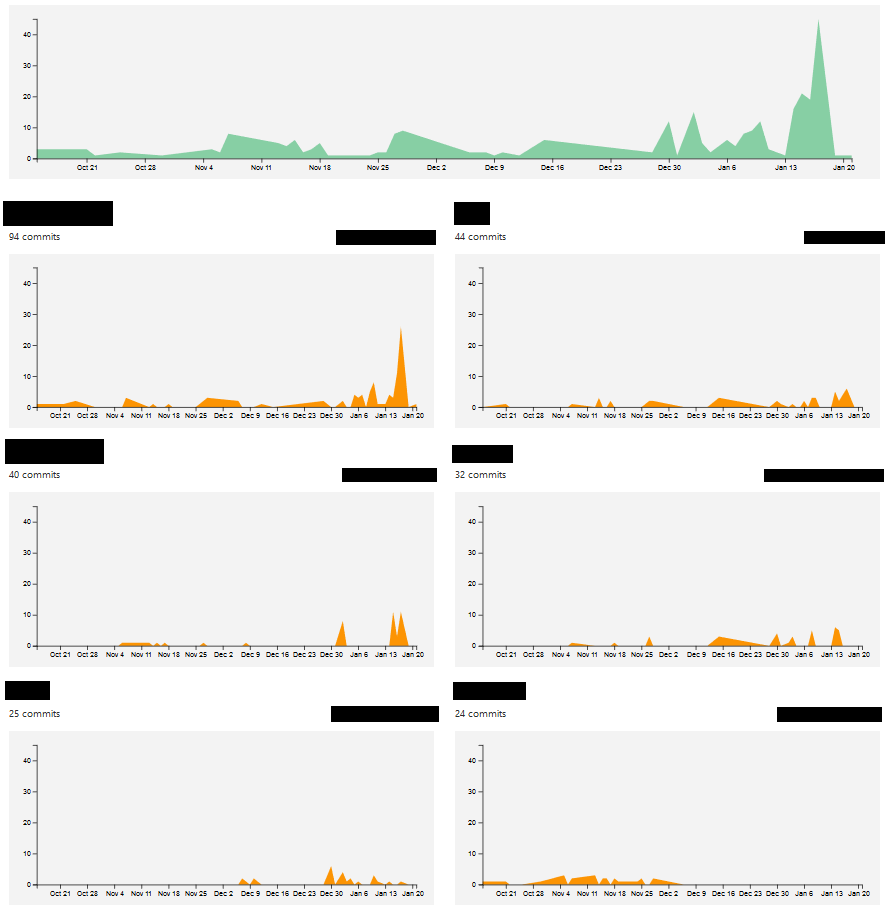
\includegraphics[scale=0.4]{slike/aktivnost.PNG} %veličina slike u odnosu na originalnu datoteku i pozicija slike
			\centering
			\caption{Primjer slike s potpisom}
			\label{fig:promjene}
		\end{figure}
		
		\begin{figure}[H]
			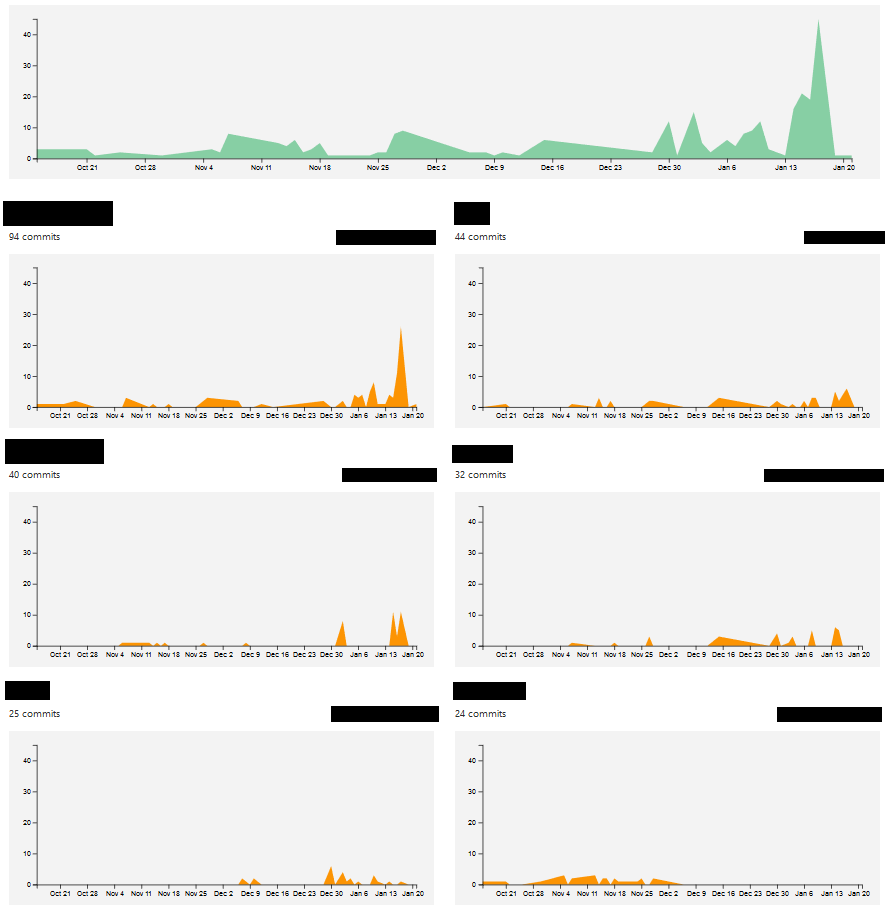
\includegraphics[width=\textwidth]{slike/aktivnost.PNG} %veličina u odnosu na širinu linije
			\caption{Primjer slike s potpisom 2}
			\label{fig:promjene2} %label mora biti drugaciji za svaku sliku
		\end{figure}
		
		Referenciranje slike \ref{fig:promjene2} u tekstu.
		
		\eject
		
	
	\chapter{Specifikacija programske potpore}
		
	\section{Funkcionalni zahtjevi}
			
			\noindent \textbf{Dionici:}
			
			\begin{packed_enum}
				
				\item Korisnik
				    \begin{packed_item}
				    \item Pacijent
				    \item Liječnik
				    \item Medicinski tehničar/sestra
				    \end{packed_item}
				\item Administrator
				\item Naručitelj
				\item Razvojni tim
			\end{packed_enum}
			
			\noindent \textbf{Aktori i njihovi funkcionalni zahtjevi:}
			
			
			\begin{packed_enum}
				
				\item  \underbar{Neregistrirani/neprijavljeni korisnik (inicijator) može:}
				
				\begin{packed_enum}
					
					\item pregledati naslovnu stranicu za neprijavljene korisnike
					\item se registrirati u sustav kao pacijent, stvoriti novi korisnicki račun za koji su mu potrebni e-mail adresa, lozinka, ime, prezime, spol, broj mobitela i odabrani liječnik
					
				\end{packed_enum}
				
				\item  \underbar{Pacijent (inicijator) može:}
				
				\begin{packed_enum}
					
					\item pregledati naslovnu stranicu za pacijente, svoj kalendar sa zakazanim pregledima i prozor za poruke o pomaknutim terminima
					\item potvrditi ili odbiti pomaknute termine
					\item odabrati pregled kod liječnika ili specifičnu vrstu usluge kod medicinskog tehničara/sestre, te zakazati termin
					\item zakazani termin otkazati
					\item dobiti podsjetnik na pregled, ili obavijest o pomaknutom pregledu na svoj e-mail ili sms
					
				\end{packed_enum}
				
				\item  \underbar{Liječnik (inicijator) može:}
				
				\begin{packed_enum}
					
					\item pregledati naslovnu stranicu za liječnike, svoj kalendar s rezerviranim terminima
					\item za rezervirane termine vidjeti tip pregleda i podatke o pacijentu
					\item definirati raspoloživost termina
					\item definirati vlastita pravila o rezervaciji termina i proizvoljno iz mijenjati
					\item pomaknuti rezervirani termin
					\item unositi potvrdu dolaska pacijenta na rezervirani termin
					
				\end{packed_enum}
				
				\item  \underbar{Medicinski tehničar/sestra (inicijator) može:}
				
				\begin{packed_enum}
					
					\item pregledati naslovnu stranicu za medicinskog tehničara, svoj kalendar sa rezerviranim terminima
					\item za rezervirane termine vidjeti vrstu specifične usluge
					\item definirati slobodne termine za specifične vrste usluga
					\item pomaknuti rezervirani termin
					\item unositi potvrdu dolaska pacijenta na rezervirani termin
					
				\end{packed_enum}
				
				\item  \underbar{Administrator (inicijator) može:}
				
				\begin{packed_enum}
					
					\item kreirati specijalizirane tipove korisnika (liječnik i medicinski tehničar/sestra)
					\item kreirati medicinske timove u kojima grupa liječnike i medicinske tehničare/sestre
					
				\end{packed_enum}
				
				\item  \underbar{Baza podataka (sudionik):}
				
				\begin{packed_enum}
					
					\item pohranjuje sve podatke o korisnicima i njihovim ovlastima
					\item pohranjuje sve podatke o zakazanim i slobodnim terminima
					
				\end{packed_enum}
				
				\item  \underbar{Sustav (sudionik):}
				
				\begin{packed_enum}
					
					\item generira izvješća o učinkovitosti rezervacije i šalje ih u informacijski sustav HZZO-a

				\end{packed_enum}
				
				
			\end{packed_enum}
			
			\eject 
			
			
				
			\subsection{Obrasci uporabe}
				
				\subsubsection{Opis obrazaca uporabe}
				
				    \noindent \underbar{\textbf{UC1 - Registracija}}
					\begin{packed_item}
	
						\item \textbf{Glavni sudionik: }Korisnik
						\item  \textbf{Cilj:} Registrirati korisnika u sustav
						\item  \textbf{Sudionici:} Baza podataka
						\item  \textbf{Preduvjet:} -
						\item  \textbf{Opis osnovnog tijeka:}
						
						\item[] \begin{packed_enum}
	
							\item Korisnik odabire opciju za registraciju
							\item Korisnik unosi potrebne podatke
							\item Pristiskom na dugme potvrđuje registraciju
							\item Po uspješnoj registraciji korisnik zaprima potvrdu na registriranu adresu e-pošte
							\item Pristup korisničkim funkcijama sukladno njegovom korisničkom tipu
						\end{packed_enum}
						
						\item  \textbf{Opis mogućih odstupanja:}
						
						\item[] \begin{packed_item}
	
							\item[2.a] Odabir već zauzetog e-maila, unos podataka u nedozvoljenom formatu ili pružanje neispravnoga e-maila 
							\item[] \begin{packed_enum}
								
								\item Sustav obavještava korisnika o neuspjelom upisu i vraća ga na stranicu za registraciju
								\item Korisnik mijenja potrebne podatke te završava unos ili odustaje od registracije
								
							\end{packed_enum}
						\end{packed_item}
					\end{packed_item}
				
				
					\noindent \underbar{\textbf{UC2 - Prijava u sustav}}
					\begin{packed_item}
	
						\item \textbf{Glavni sudionik: }Korisnik
						\item  \textbf{Cilj:} Prijaviti korisnika u sustav
						\item  \textbf{Sudionici:} Baza podataka
						\item  \textbf{Preduvjet:} Registracija
						\item  \textbf{Opis osnovnog tijeka:}
						
						\item[] \begin{packed_enum}
	                        
	                        \item Korisnik odabire opciju za prijavu
							\item Unos korisničkog imena i lozinke
							\item Pristiskom na dugme potvrđuje prijavu
							\item Pristup korisničkim funkcijama sukladno njegovom korisničkom tipu
						\end{packed_enum}
						
						\item  \textbf{Opis mogućih odstupanja:}
						
						\item[] \begin{packed_item}
	
							\item[2.a] Neispravno korisničko ime/lozinka
							\item[] \begin{packed_enum}
								
								\item Sustav obavještava korisnika o neuspjelom upisu i vraća ga na stranicu za prijavu
								\item Korisnik mijenja potrebne podatke te završava unos ili odustaje od prijave
							\end{packed_enum}
						\end{packed_item}
					\end{packed_item}
					
					\noindent \underbar{\textbf{UC3 - Pregled zakazanih termina}}
					\begin{packed_item}
	
						\item \textbf{Glavni sudionik: } Pacijent
						\item  \textbf{Cilj:} Omogućiti pacijentu uvid u zakazane termine
						\item  \textbf{Sudionici:} Baza podataka
						\item  \textbf{Preduvjet:} Korisnik prijavljen kao pacijent
						\item  \textbf{Opis osnovnog tijeka:}
						
						\item[] \begin{packed_enum}
	
							\item Korisniku se prikaže naslovna stranica za pacijente
							\item Korisnik na vlastitom kalendaru ima uvid u svoje termine
						\end{packed_enum}
						
					\end{packed_item}
					
					\noindent \underbar{\textbf{UC4 - Zakazivanje termina kod liječnika}}
					\begin{packed_item}
	
						\item \textbf{Glavni sudionik: }Pacijent
						\item  \textbf{Cilj:} Omogućiti pacijentu odabir termina pregleda kod liječnika
						\item  \textbf{Sudionici:} Baza podataka
						\item  \textbf{Preduvjet:} Prijavljen korisnik kao pacijent
						\item  \textbf{Opis osnovnog tijeka:}
						
						\item[] \begin{packed_enum}
	
							\item Korisniku se prikaže naslovna stranica za pacijente
							\item Korisnik odabire opciju zakazivanja pregleda kod liječnika 
							\item Na prikazanom kalendaru odabire željeni slobodni termin
							\item Dodatno naznačuje tip pregleda
							\item Pristiskom na dugme potvrđuje odabrani termin
							\item Korisnik dobiva potvrdu o uspješno odabranom terminu na preferirani kanal komunikacije
							\item Korisnikov kalendar se osvježava novim podacima
						\end{packed_enum}
						
						\item  \textbf{Opis mogućih odstupanja:}
						
						\item[] \begin{packed_item}
	
							\item[2.a] Korisnik je previše puta rezervirao termine
							\item[] \begin{packed_enum}
								
								\item Sustav onemogućuje zakazivanje termina i korisniku šalje odgovarajuću poruku
								\item Korisnik je preusmjeren natrag na svoju naslovnu stranicu
							\end{packed_enum}
							
							\item[2.b] Korisnik se previše puta nije pojavio na zakazanom terminu
							\item[] \begin{packed_enum}
								
								\item Sustav onemogućuje zakazivanje termina i korisniku šalje odgovarajuću poruku
								\item Korisnik je preusmjeren natrag na svoju naslovnu stranicu
							\end{packed_enum}
						\end{packed_item}
					\end{packed_item}
					
					\noindent \underbar{\textbf{UC5 - Zakazivanje termina kod medicinskog tehničara}}
					\begin{packed_item}
	
						\item \textbf{Glavni sudionik: }Pacijent
						\item  \textbf{Cilj:} Omogućiti pacijentu odabir termina usluge kod medicinskog tehničara
						\item  \textbf{Sudionici:} Baza podataka
						\item  \textbf{Preduvjet:} Prijavljen korisnik kao pacijent
						\item  \textbf{Opis osnovnog tijeka:}
						
						\item[] \begin{packed_enum}
	
							\item Korisniku se prikaže naslovna stranica za pacijente
							\item Korisnik odabire zakazivanje pregleda kod medicinskog tehničara
							\item Korisnik odabire vrstu usluge unutar predefiniranih termina
							\item Pristiskom na dugme potvrđuje odabranu uslugu
							\item Sustav korisniku dodjeljuje prvi slobodni termin
							\item Korisnik dobiva potvrdu o uspješno odabranom terminu na preferirani kanal komunikacije
							\item Korisnikov kalendar se osvježava novim podacima
						\end{packed_enum}
						
						\item  \textbf{Opis mogućih odstupanja:}
						
						\item[] \begin{packed_item}
	
							\item[2.a] Korisnik je previše puta rezervirao termine
							\item[] \begin{packed_enum}
								
								\item Sustav onemogućuje zakazivanje termina i korisniku šalje odgovarajuću poruku
								\item Korisnik je preusmjeren natrag na svoju naslovnu stranicu
							\end{packed_enum}
							
							\item[2.b] Korisnik se previše puta nije pojavio na zakazanom terminu
							\item[] \begin{packed_enum}
								
								\item Sustav onemogućuje zakazivanje termina i korisniku šalje odgovarajuću poruku
								\item Korisnik je preusmjeren natrag na svoju naslovnu stranicu
							\end{packed_enum}
						\end{packed_item}
					\end{packed_item}
					
					
					\noindent \underbar{\textbf{UC6 - Otkazivanje termina}}
					\begin{packed_item}
	
						\item \textbf{Glavni sudionik: }Pacijent
						\item  \textbf{Cilj:} Omogućiti pacijentu otkazivanje termina
						\item  \textbf{Sudionici:} Baza podataka
						\item  \textbf{Preduvjet:} Prijavljen korisnik kao pacijent,  postoji zakazan pregled
						\item  \textbf{Opis osnovnog tijeka:}
						
						\item[] \begin{packed_enum}
	
							\item Korisniku se prikaže naslovna stranicu za pacijente
							\item Korisnik na prikazanom kalendaru odabire zakazani termin
							\item Korisnik odabire opciju za otkazivanje pregleda
							\item Pristiskom na dugme potvrđuje odabranu opciju
							\item Korisnik dobiva potvrdu o uspješno otkazanom terminu na preferirani kanal komunikacije
							\item Korisnikov kalendar se osvježava novim podacima
							
						\end{packed_enum}
						
						\item  \textbf{Opis mogućih odstupanja:}
						
						\item[] \begin{packed_item}
	
							\item[2.a] Korisnik je pokušao otkazati termin 24 sata nakon zakazivanja
							\item[] \begin{packed_enum}
								
								\item Sustav onemogućuje otkazivanje i korisniku šalje odgovarajuću poruku
								\item Korisnik je preusmjeren natrag na svoju naslovnu stranicu
								
							\end{packed_enum}
						\end{packed_item}
						
					\end{packed_item}
					
					
					
					\noindent \underbar{\textbf{UC7 - Potvrđivanje novih termina nakon pomicanja}}
					\begin{packed_item}
	
						\item \textbf{Glavni sudionik: }Pacijent
						\item  \textbf{Cilj:} Pacijentu omogućiti potvrdu ili odbijanje novog termina
						\item  \textbf{Sudionici:} Baza podataka
						\item  \textbf{Preduvjet:} Korisnik prikavljen kao pacijent, liječniki tim je pomaknuo zakazani termin
						\item  \textbf{Opis osnovnog tijeka:}
						
						\item[] \begin{packed_enum}
	                        
	                        \item Sustav korisniku šalje poruku o promjenjenom terminu
							\item Korisniku se prikaže naslovna stranicu za pacijente
							\item Korisniku se u posebnom prozoru prikaže poruka o promjeni uz opcije prihvaćanja promjene
							\item Korisnik odabire opciju za prihvačanje novog termina
							\item Pristiskom na dugme potvrđuje odabranu opciju
							\item Korisnik dobiva potvrdu o uspješno prihvačenom ili odbijenom terminu na preferirani kanal komunikacije
							\item Korisnikov kalendar se osvježava novim podacima
						\end{packed_enum}
						
					
					\end{packed_item}
					
					\noindent \underbar{\textbf{UC8 - Podsjećanje pacijenta na zakazani termin}}
					\begin{packed_item}
	
						\item \textbf{Glavni sudionik: }-
						\item  \textbf{Cilj:} Slanje podsjetnika pacijentu na termin
						\item  \textbf{Sudionici:} Baza podataka, pacijent
						\item  \textbf{Preduvjet:} Postoji zakazani termin
						\item  \textbf{Opis osnovnog tijeka:}
						
						\item[] \begin{packed_enum}
	
							\item Prikupljanje podataka o pregledu i preferiranom kanalu komunikacije
							\item Konverzija u željeni oblik
							\item Slanje podsjetnika pacijentu putem preferiranog kanala komunikacije
						\end{packed_enum}
						
						\item  \textbf{Opis mogućih odstupanja:}
						
						\item[] \begin{packed_item}
	
							\item[3.a] Sustav nije mogao poslati podsjetnik zbog greške u e-mail/sms sustavu
							\item[] \begin{packed_enum}
								
								\item Sustav šalje podsjetnik putem opcionalnog kanala komunikacije
						
							\end{packed_enum}
							
						\end{packed_item}
					\end{packed_item}
					
					\noindent \underbar{\textbf{UC9 - Pregled rezeviranih termina}}
					\begin{packed_item}
	
						\item \textbf{Glavni sudionik: } Liječnik, medicinski tehničar
						\item  \textbf{Cilj:} Omogućiti medicinskom osoblju uvid u zakazane termine s dodatnim informacijama
						\item  \textbf{Sudionici:} Baza podataka
						\item  \textbf{Preduvjet:} Korisnik prijavljen kao liječnik ili medicinski tehničar
						\item  \textbf{Opis osnovnog tijeka:}
						
						\item[] \begin{packed_enum}
	
							\item Korisniku se prikaže naslovna stranica za liječnike ili medicinske tehničare
							\item Pritiskom na željeni termin u kalenadru korisnik dobije više informacija
							
						\end{packed_enum}
					\end{packed_item}
					
					\noindent \underbar{\textbf{UC10 - Potvrđivanje dolaznosti pacijenta}}
					\begin{packed_item}
	
						\item \textbf{Glavni sudionik: } Liječnik, medicinski tehničar
						\item  \textbf{Cilj:} Omogućiti medicinskom osoblju potvrđivanje dolaznosti pacijenta
						\item  \textbf{Sudionici:} Baza podataka
						\item  \textbf{Preduvjet:} Korisnik prijavljen kao liječnik ili medicinski tehničar, završio zakazani termin
						\item  \textbf{Opis osnovnog tijeka:}
						
						\item[] \begin{packed_enum}
	
							\item Korisniku se prikaže naslovna stranica za liječnike ili medicinske tehničare
							\item Pritiskom na željeni termin u kalenadru korisnik dobije više informacija
							\item Korisnik obabire opciju za potvrđivanjem dolaznosti pacijenta
							
						\end{packed_enum}
					\end{packed_item}
					
					\noindent \underbar{\textbf{UC11 - Definiranje raspoloživosti termina}}
					\begin{packed_item}
	
						\item \textbf{Glavni sudionik: } Liječnik
						\item  \textbf{Cilj:} Omogućiti liječniku definiranje raspoživosti termina 10 dana unaprijed
						\item  \textbf{Sudionici:} Baza podataka
						\item  \textbf{Preduvjet:} Korisnik prijavljen kao liječnik
						\item  \textbf{Opis osnovnog tijeka:}
						
						\item[] \begin{packed_enum}
	
							\item Korisniku se prikaže naslovna stranica za liječnike
							\item Korisnik bira opciju za uređivanje raspoloživosti termina
							\item Korisnik za 10 dana unaprijed definira raspoloživost termina
							\item Korisnik pritiskom na dugme sprema promjene
							\item Korisnikov kalendar se osvježava novim podacima
							
						\end{packed_enum}
					\end{packed_item}
					
					\noindent \underbar{\textbf{UC12 - Definiranje vlastitih pravila o rezervaciji termina}}
					\begin{packed_item}
	
						\item \textbf{Glavni sudionik: } Liječnik
						\item  \textbf{Cilj:} Omogućiti liječniku definiranje vlastita pravila o rezervaciji termina
						\item  \textbf{Sudionici:} Baza podataka
						\item  \textbf{Preduvjet:} Korisnik prijavljen kao liječnik
						\item  \textbf{Opis osnovnog tijeka:}
						
						\item[] \begin{packed_enum}
	
							\item Korisniku se prikaže naslovna stranica za liječnike
							\item Korisnik bira opciju za uređivanje vlastitih pravila o rezervaciji termina
							\item Korisnik na padajućem izborniku bira koliko sati unaprijed pacijent mora rezervirati termin
							\item Korisnik pritiskom na dugme sprema promjene
							
						\end{packed_enum}
					\end{packed_item}
					
					\noindent \underbar{\textbf{UC13 - Definiranje termina za specifične vrste usluga}}
					\begin{packed_item}
	
						\item \textbf{Glavni sudionik: } Medicinski tehničar/sestra
						\item  \textbf{Cilj:} Omogućiti medicinskom tehničaru definiranje slobodnih termina za specifične vrste usluga
						\item  \textbf{Sudionici:} Baza podataka
						\item  \textbf{Preduvjet:} Korisnik prijavljen kao medicinski tehničar
						\item  \textbf{Opis osnovnog tijeka:}
						
						\item[] \begin{packed_enum}
	
							\item Korisniku se prikaže naslovna stranica za medicinske tehničare
							\item Korisnik bira opciju za uređivanje slobodnih termina
							\item Korisnik za 10 dana unaprijed definira slobodne termine za specifične vrste usluga
							\item Korisnik pritiskom na dugme sprema promjene
							\item Korisnikov kalendar se osvježava novim podacima
						\end{packed_enum}
					\end{packed_item}
					
					\noindent \underbar{\textbf{UC14 - Pomicanje zakazanih termina}}
					\begin{packed_item}
	
						\item \textbf{Glavni sudionik: } Medicinski tehničar/sestra, Liječnik
						\item  \textbf{Cilj:} Omogućiti medicinskom tehničaru ili liječniku pomicanje zakazanog termina do 24 sata nakon rezervacije
						\item  \textbf{Sudionici:} Baza podataka
						\item  \textbf{Preduvjet:} Korisnik prijavljen kao medicinski tehničar ili liječnik
						\item  \textbf{Opis osnovnog tijeka:}
						
						\item[] \begin{packed_enum}
	
							\item Korisniku se prikaže naslovna stranica za medicinske tehničare ili liječnike
							\item Korisnik na vlastitom kalendaru bira termin koji želi pomaknuti
							\item Korisnik odabire opciju za mijenjanje termina i bira novi termin
							\item Korisnik pritiskom na dugme sprema promjene
							\item Korisnikov kalendar se osvježava novim podacima
							
						\end{packed_enum}
						\item  \textbf{Opis mogućih odstupanja:}
						
						\item[] \begin{packed_item}
	
							\item[2.a] Korisnik je odabrao termin od čije je rezervacije prošlo više od 24 sata
							\item[] \begin{packed_enum}
								
								\item Sustav onemogućuje pomicanje termina i korisniku šalje odgovarajuću poruku
								\item Korisnik je preusmjeren natrag na svoju naslovnu stranicu
						
							\end{packed_enum}
							
						\end{packed_item}
					\end{packed_item}
					
					\noindent \underbar{\textbf{UC15 - Stvaranje liječnika}}
					\begin{packed_item}
	
						\item \textbf{Glavni sudionik: } Administrator
						\item  \textbf{Cilj:} Omogućiti administratoru stvaranje specijaliziranog tipa korisnika - liječnika, s omogučenim posebinim aktivnostima
						\item  \textbf{Sudionici:} Baza podataka
						\item  \textbf{Preduvjet:} Korisnik prijavljen kao administrator
						\item  \textbf{Opis osnovnog tijeka:}
						
						\item[] \begin{packed_enum}
	
							\item Korisniku se prikaže naslovna stranica za administratore
							\item Korisnik bira opciju za stvaranje liječnika
							\item U formi unosi podatke o novom liječniku
							\item Korisnik pritiskom na dugme sprema promjene
							
						\end{packed_enum}
						
						\item  \textbf{Opis mogućih odstupanja:}
						\item[] \begin{packed_item}
						
							\item[2.a] Odabir već zauzetog e-maila, unos podataka u nedozvoljenom formatu ili pružanje neispravnoga e-maila 
							\item[] \begin{packed_enum}
								
								\item Sustav obavještava korisnika o neuspjelom upisu i vraća ga na stranicu za staranje novog liječnika
								\item Korisnik mijenja potrebne podatke te završava unos ili odustaje od stvaranja novog liječnika
								
							\end{packed_enum}
						\end{packed_item}
					\end{packed_item}
					
					\noindent \underbar{\textbf{UC16 - Stvaranje medicinskog tehničara/sestre}}
					\begin{packed_item}
	
						\item \textbf{Glavni sudionik: } Administrator
						\item  \textbf{Cilj:} Omogućiti administratoru stvaranje specijaliziranog tipa korisnika - medicinskog tehničara/sestre, s omogučenim posebinim aktivnostima
						\item  \textbf{Sudionici:} Baza podataka
						\item  \textbf{Preduvjet:} Korisnik prijavljen kao administrator
						\item  \textbf{Opis osnovnog tijeka:}
						
						\item[] \begin{packed_enum}
	
							\item Korisniku se prikaže naslovna stranica za administratore
							\item Korisnik bira opciju za stvaranje medicinskog tehničara
							\item U formi unosi podatke o novom medicinskom tehničaru
							\item Korisnik pritiskom na dugme sprema promjene
							
						\end{packed_enum}
						
						\item  \textbf{Opis mogućih odstupanja:}
							
						\item[] \begin{packed_item}
						
							\item[2.a] Odabir već zauzetog e-maila, unos podataka u nedozvoljenom formatu ili pružanje neispravnoga e-maila 
							\item[] \begin{packed_enum}
								
								\item Sustav obavještava korisnika o neuspjelom upisu i vraća ga na stranicu za staranje novog medicinskog tehničara
								\item Korisnik mijenja potrebne podatke te završava unos ili odustaje od stvaranja novog medicinskog tehničara
								
							\end{packed_enum}
						\end{packed_item}
					\end{packed_item}
					
				
					
					\noindent \underbar{\textbf{UC17 - Pregled medicinskih timova}}
					\begin{packed_item}
	
						\item \textbf{Glavni sudionik: } Administrator
						\item  \textbf{Cilj:} Omogućiti administratoru pregled medicinskih timova
						\item  \textbf{Sudionici:} Baza podataka
						\item  \textbf{Preduvjet:} Korisnik prijavljen kao administrator
						\item  \textbf{Opis osnovnog tijeka:}
						
						\item[] \begin{packed_enum}
	
							\item Korisniku se prikaže naslovna stranica za administratore
							\item Korisnik bira opciju za pregled medicinskog timova
							
						\end{packed_enum}
					\end{packed_item}
					
					\noindent \underbar{\textbf{UC18 - Brisanje medicinskog tima}}
					\begin{packed_item}
	
						\item \textbf{Glavni sudionik: } Administrator
						\item  \textbf{Cilj:} Omogućiti administratoru brisanje medicinskog tima, čime medicinsko osoblje čini slobodnim za grupiranje
						\item  \textbf{Sudionici:} Baza podataka
						\item  \textbf{Preduvjet:} Korisnik prijavljen kao administrator, u bazi postoji barem jedan medicinski tim
						\item  \textbf{Opis osnovnog tijeka:}
						
						\item[] \begin{packed_enum}
	
							\item Korisniku se prikaže naslovna stranica za administratore
							\item Korisnik bira opciju za pregled medicinskih timova
							\item Korisnik za odabarni tim pritisne brisanje tima
							\item Korisnik pritiskom na dugme sprema promjene
							\item Korisnikov popis timova se osvježi novim podacima
							
						\end{packed_enum}
					\end{packed_item}
					
					\noindent \underbar{\textbf{UC19 - Stvaranje novog medicinskog tima}}
					\begin{packed_item}
	
						\item \textbf{Glavni sudionik: } Administrator
						\item  \textbf{Cilj:} Omogućiti administratoru grupiranje liječnika i medicinskog tehničara u medicinski tim
						\item  \textbf{Sudionici:} Baza podataka
						\item  \textbf{Preduvjet:} Korisnik prijavljen kao administrato, u bazi postoji barem jedan liječnik i medicinski tehničar
						\item  \textbf{Opis osnovnog tijeka:}
						
						\item[] \begin{packed_enum}
	
							\item Korisniku se prikaže naslovna stranica za administratorea
							\item Korisnik bira opciju za stvaranje novog medicinskog tima
							\item U formi unosi imena liječnika i medicinskog tehničara koje želi grupirati
							\item Korisnik pritiskom na dugme sprema promjene
							
						\end{packed_enum}
						
						\item  \textbf{Opis mogućih odstupanja:}
						\item[] \begin{packed_item}
						
							\item[2.a] Korisnik je odabrao liječnika ili medicinskog tehničara koji već je u nekom timu
							\item[] \begin{packed_enum}
								
								\item Sustav onemogćuje stvaranje tima i korisniku šalje odgovarajuću poruku
								\item Korisnik je preusmjeren natrag na stvaranje novog tima
								
							\end{packed_enum}
						\end{packed_item}
					\end{packed_item}
					
					\noindent \underbar{\textbf{UC20 - Generiranje izvješća}}
					\begin{packed_item}
	
						\item \textbf{Glavni sudionik: } -
						\item  \textbf{Cilj:} Generiranje dnevnih i mjesečnih izvješća i slanje u informacijski sustav HZZO-a
						\item  \textbf{Sudionici:} Baza podataka, HZZO
						\item  \textbf{Preduvjet:} -
						\item  \textbf{Opis osnovnog tijeka:}
						
						\item[] \begin{packed_enum}
	
							\item Prikupljanje podataka unesenih u proteklom razdoblju
							\item Konverzija podataka u željeni oblik
							\item Slanje podataka HZZO-u
							
						\end{packed_enum}
						
						\item  \textbf{Opis mogućih odstupanja:}
						\item[] \begin{packed_item}
						
							\item[2.a] Informacijski sustav HZZO-a nije dostupan
							\item[] \begin{packed_enum}
								
								\item Sustav čeka 1 sat i pokušava ponovo
								
							\end{packed_enum}
						\end{packed_item}
					\end{packed_item}
					
					
				\newpage
					
				\subsubsection{Dijagrami obrazaca uporabe}
							
				
					\begin{figure}[H]
			            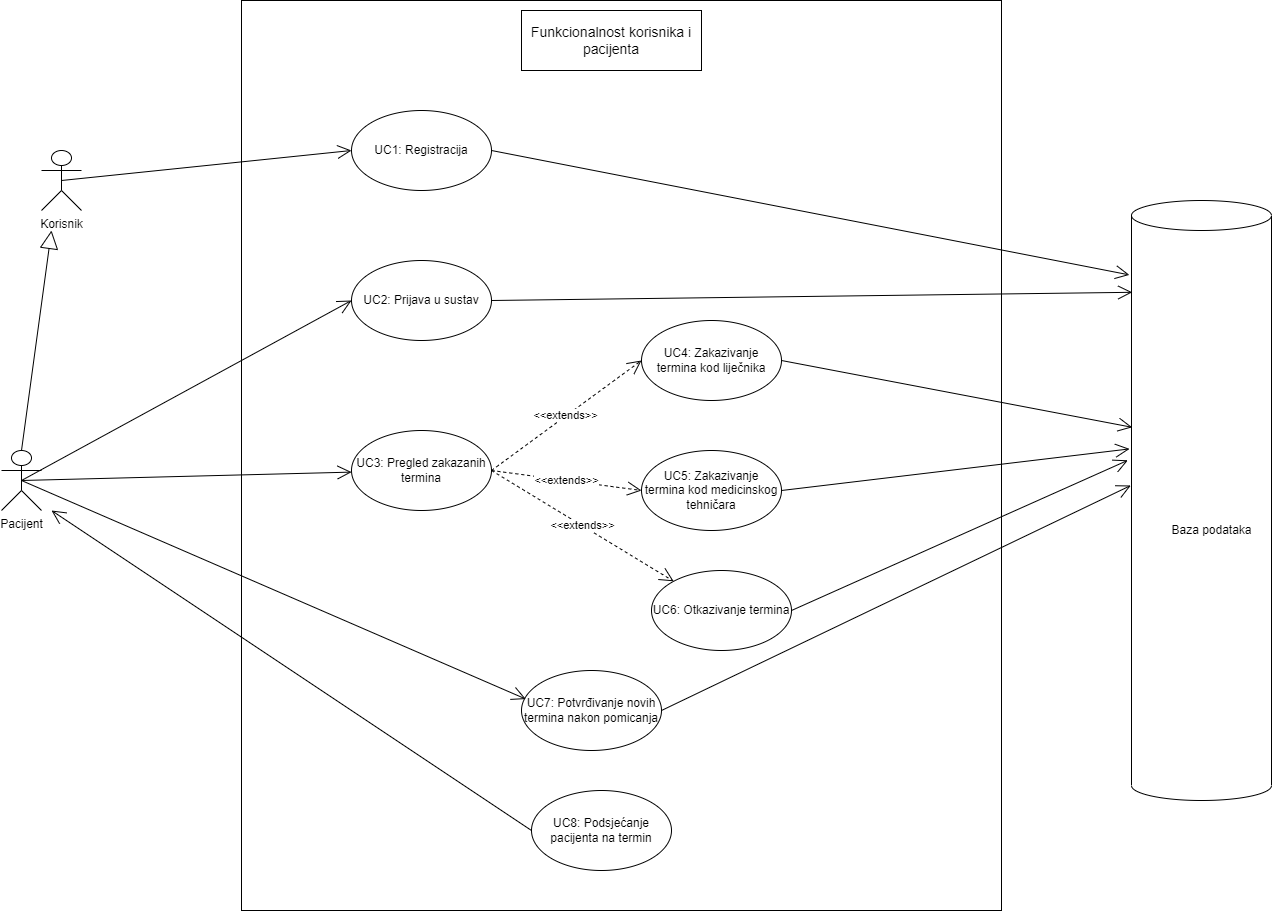
\includegraphics[width=\textwidth]{slike/pacijent_usecase.png} %veličina u odnosu na širinu linije
			            \caption{Dijagram obrasca uporabe, funkcionalnost korisnika i pacijenta}
			            \label{fig:promjene2} %label mora biti drugaciji za svaku sliku
		            \end{figure}
				
				    \begin{figure}[H]
			            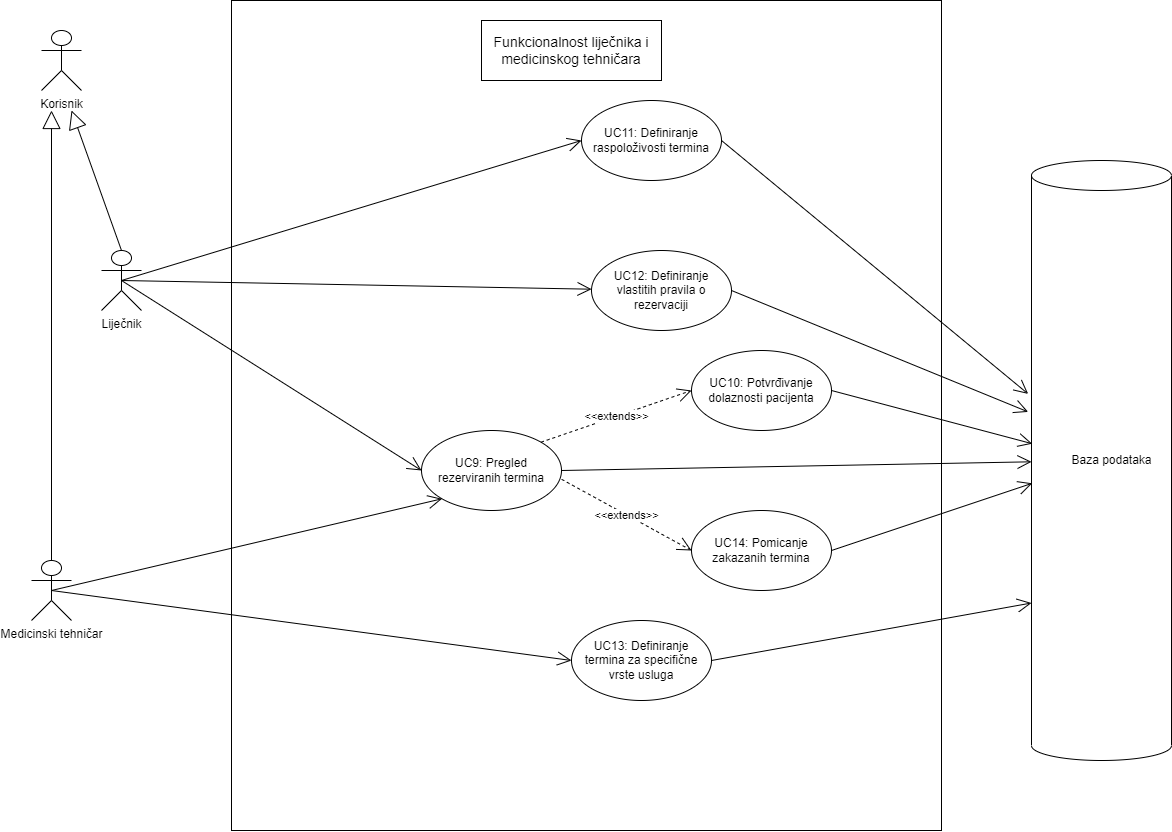
\includegraphics[width=\textwidth]{slike/lijecnik_tehn_usecase.png} %veličina u odnosu na širinu linije
			            \caption{Dijagram obrasca uporabe, funkcionalnost liječnika i medicinskog tehničara/sestre}
			            \label{fig:promjene2} %label mora biti drugaciji za svaku sliku
		            \end{figure}
				
				    \begin{figure}[H]
			            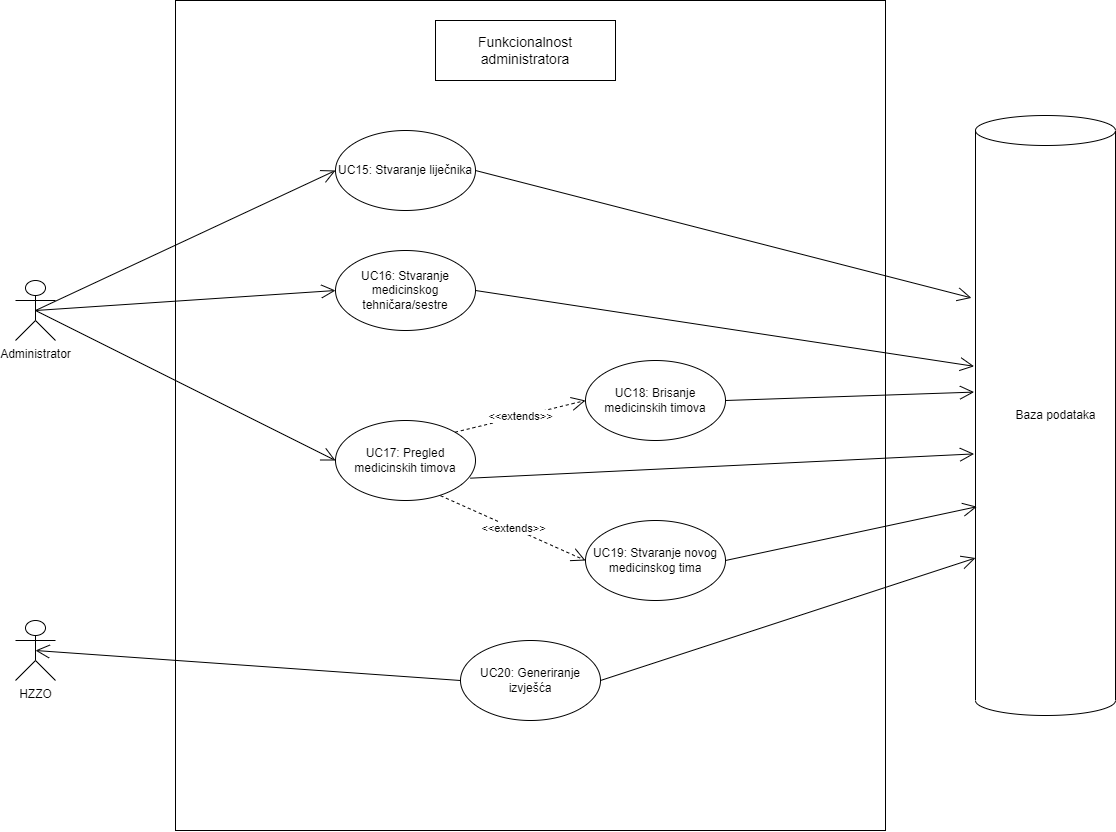
\includegraphics[width=\textwidth]{slike/administrator_usecase.png} %veličina u odnosu na širinu linije
			            \caption{Dijagram obrasca uporabe, funkcionalnost administratora}
			            \label{fig:promjene2} %label mora biti drugaciji za svaku sliku
		            \end{figure}
		            
		            \eject
		            
			\subsection{Sekvencijski dijagrami}
				
				\subsubsection{Obrazac uporabe UC4 - Zakazivanje termina kod liječnika}
				Korisnik, prijavljen kao pacijent, želi vidjeti kalendar sa svojim terminima kako bi mogao zakazati sljedeći termin. Poslužitelj dohvaća trenutne termine i prikazuje ih. Korisnik želi zatražiti novi termin kod liječnika, međutim poslužitelj najprije mora provjeriti koji je status korisnika. Ako je sve u redu, pacijent je redovan, i poslužitelj dohvaća slobodne termine korisnikovog liječnika iz baze podataka i prikazuje ih korisniku. Korisnik bira željeni termin i dodatno naznačuje tip pregleda. Poslužitelj šalje nove podatke u bazu te obavještava korisnika te mu osvježava  kalendar. Ako je u korisnikovom statusu označeno da ima previše izostanaka sa zakazanih termina ili je zakazao previše termina, poslužitelj odbija zakazati novi termin i šalje odgovarajuću poruku korisniku.
				
				
				\begin{figure}[H]
			            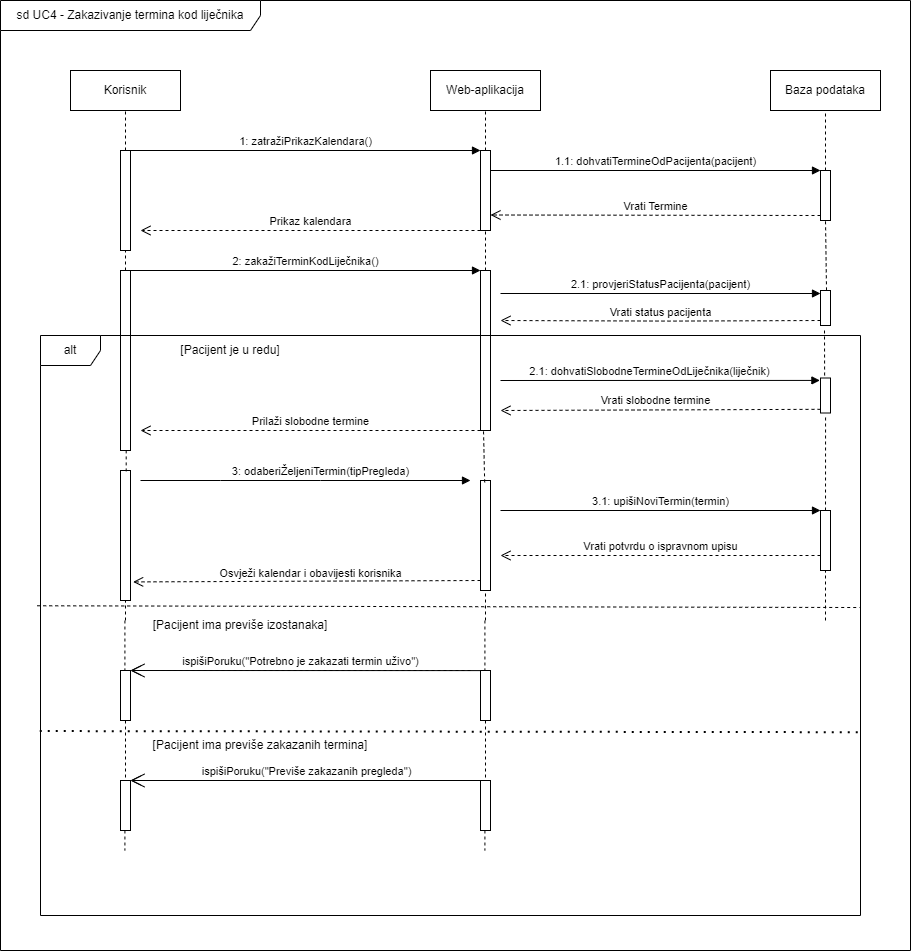
\includegraphics[width=\textwidth]{slike/sd_uc4.png} %veličina u odnosu na širinu linije
			            \caption{Sekvencijski dijagram za UC4}
			            \label{fig:promjene2} %label mora biti drugaciji za svaku sliku
		            \end{figure}
		            
		        \eject
				
				\subsubsection{Obrazac uporabe UC6 - Otkazivanje termina}
				
				Korisnik, prijavljen kao pacijent, želi vidjeti kalendar sa svojim terminima kako bi mogao otkazati sljedeći termin. Poslužitelj dohvaća trenutne termine i prikazuje ih. Korisnik želi otkazati termin te na svom kalendaru pronalazi željeni termin i otkazuje ga. Poslužitelj tada najprije provjera koliko je vremena prošlo od rezervacije zadanog termina. Ako je prošlo više od 24 sata, tada poslužitelj odbija otkazati termin uz odgovarajuću poruku korisniku. Inače, poslužitelj šalje bazi podatak o terminu kojeg treba obrisati, te na potvrdu baze o uspješnom brisanju obavještava korisnika i osvježava mu kalendar.
				
				\begin{figure}[H]
			            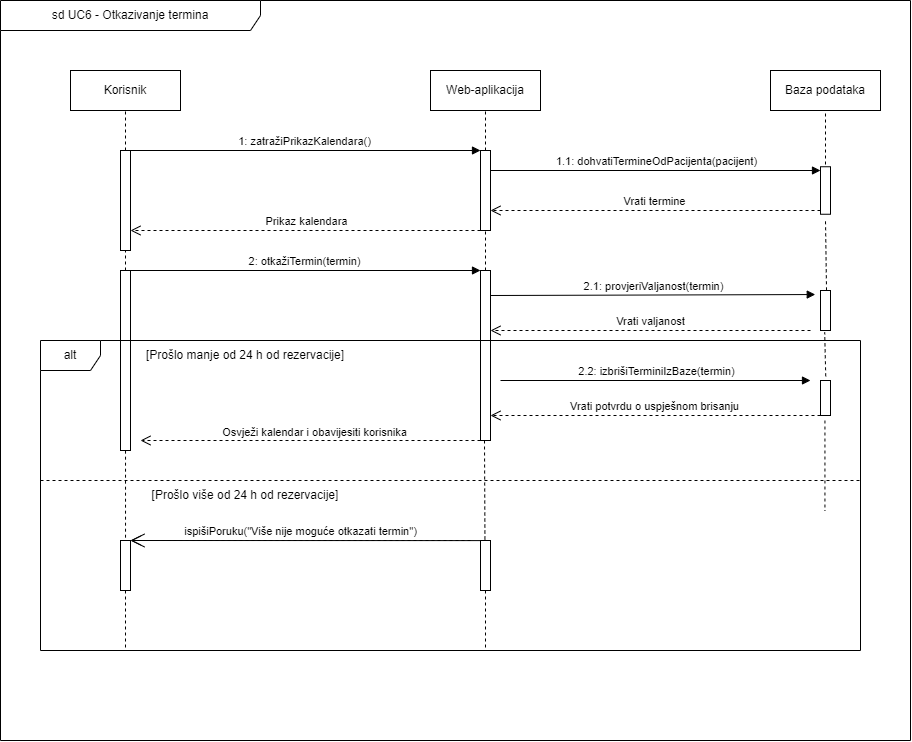
\includegraphics[width=\textwidth]{slike/sd_uc6.png} %veličina u odnosu na širinu linije
			            \caption{Sekvencijski dijagram za UC6}
			            \label{fig:promjene2} %label mora biti drugaciji za svaku sliku
		        \end{figure}
		            
		        \eject
		            
		            
				\subsubsection{Obrazac uporabe UC11 - Definiranje raspoloživosti termina}
				
				Korisnik, prijavljen kao liječnik, želi vidjeti kalendar kako bi imao uvid u svoje termine i mogao definirati njihovu raspoloživost. Poslužitelj dohvaća trenutne termine i prikazuje ih. Nakon što korisnik odluči definirati termine, poslužitelj mu vraća formu koja mu to omogućuje. Korisnik ima mogućnost definiranja termina sve dok ne potvrdi promjene. Nakon što korisnik potvrdi promjene, poslužitelj signalizira bazi da ih spremi. Poslije potvrde baze, poslužitelj osvježava korisnikov kalendar.
				
				\begin{figure}[H]
			            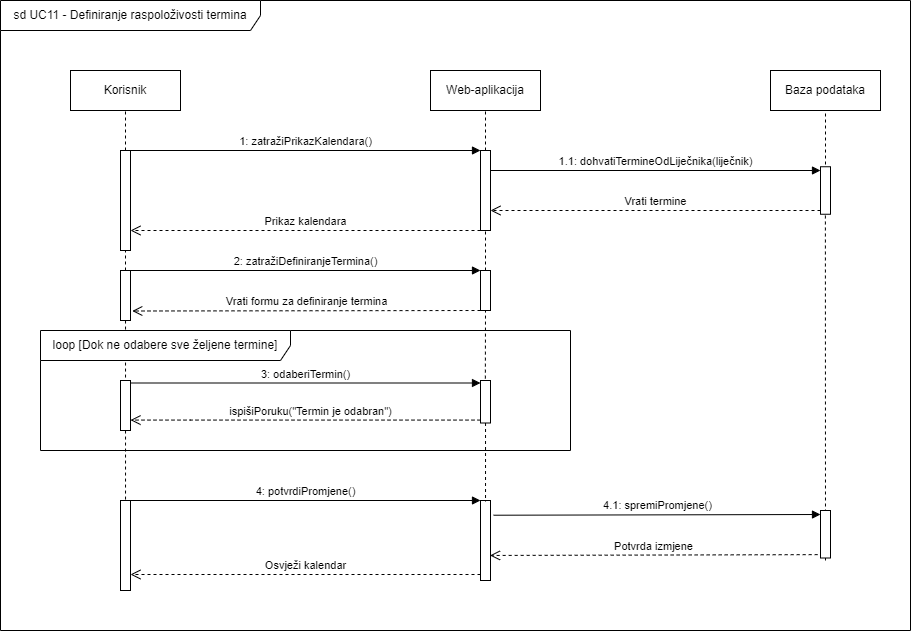
\includegraphics[width=\textwidth]{slike/sd_uc11.png} %veličina u odnosu na širinu linije
			            \caption{Sekvencijski dijagram za UC11}
			            \label{fig:promjene2} %label mora biti drugaciji za svaku sliku
		        \end{figure}
		        
		        \eject

		\section{Ostali zahtjevi}
			
			 \begin{packed_item}
			     \item Sustav treba biti izveden kao web aplikacija kojoj će korisnici pristupati uz pomoć korisničkog imena i lozinke
			     \item Oblikovanje aplikacije mora slijediti načela objektno-orijentiranog programiranja
			     \item Aplikacija treba biti jednostavna za korištenje, a sučelje pregledno i intuitivno
			     \item  Korisničko sučelje i sustav moraju podržavati hrvatsku abecedu (dijakritičke znakove) pri unosu i prikazu tekstualnog sadržaja
			     \item Sustav treba podržavati rad više korisnika u stvarnom vremenu
			     \item Neispravno korištenje korisničkog sučelja ne smije narušiti funkcionalnost i rad sustava
			     \item Veza s bazom podataka mora biti kvalitetno zastičena, brza i otporna na vanjske greške
			     \item Generirana dnevna i mjesečna izvješća o učinkovitosti šalju se u XML formatu
			     
			 \end{packed_item}
			 
			 
			 
	
	\chapter{Arhitektura i dizajn sustava}
		\texttt{}{ Arhitekturu projektnog sustava možemo podijeliti u 3 cjeline:}
	\begin{itemize}
		\item 	\textit{Web aplikacija }
		\item 	\textit{Web poslužitelj}
		\item 	\textit{Baza podataka }		
	\end{itemize}


                \texttt{}{
             Web preglednik je dio arhitekture koji korisniku omogućuje pregled web stranice i svih sadržaja na njoj. Svaki internetski preglednik je prevoditelj. Korisnik putem web preglednika šalje zahtjev web poslužitelju. 
            }

            
                \texttt{}{
             Web poslužitelj osnova je rada web aplikacije. Njegov primaran zadatak je komunikacija klijenta s aplikacijom. Komunikacija se odvija preko HTTP (engl. Hyper Text Transfer Protocol) protokola, sto je protokol u prijenosu informacija na webu. Poslužitelj je onaj koji pokreće web aplikaciju te joj prosljeđuje zahtjev
            }


            
                \texttt{}{
            Korisnik koristi web aplikaciju za obrađivanje željenih zahtijeva. Web aplikacija obrađuje zahtjev te ovisno o zahtjevu, pristupa bazi podataka nakon čega preko poslužitelja vraća korisniku odgovor u obliku HTML dokumenta vidljivog u web pregledniku.}
               

                \texttt{}{
             Null grupa 2022./2023. za projekt na predmetu Programsko inženjerstvo 2022./2023. odabrala je Angular sustav za izradu frontenda (dijela sustava vidljivoga korisniku) i Express sustav za izradu backenda (dijela sustava koji nije vidljiv korisniku) projetknog zadatka. 
            Arhitektura AngularJS-a temelji se na MVC dizajnu (Model, view, controller).
            Model View Controller ili MVC kako se popularno naziva, uzorak je dizajna softvera za razvoj web aplikacija. MVC dizajn sastoji se od sljedeća tri dijela:
            }
            \begin{itemize}
		\item 	\text{ Model je najniža razina uzorka odgovornog za održavanje podataka. }
		\item 	\text{ Prikaz(view) odgovoran je za prikazivanje svih ili dijela podataka korisniku.}
		\item 	\text{Kontroler je softverski kod koji kontrolira interakcije između modela i prikaza.}		
	\end{itemize}
        \eject

             \begin{figure}[H]
			            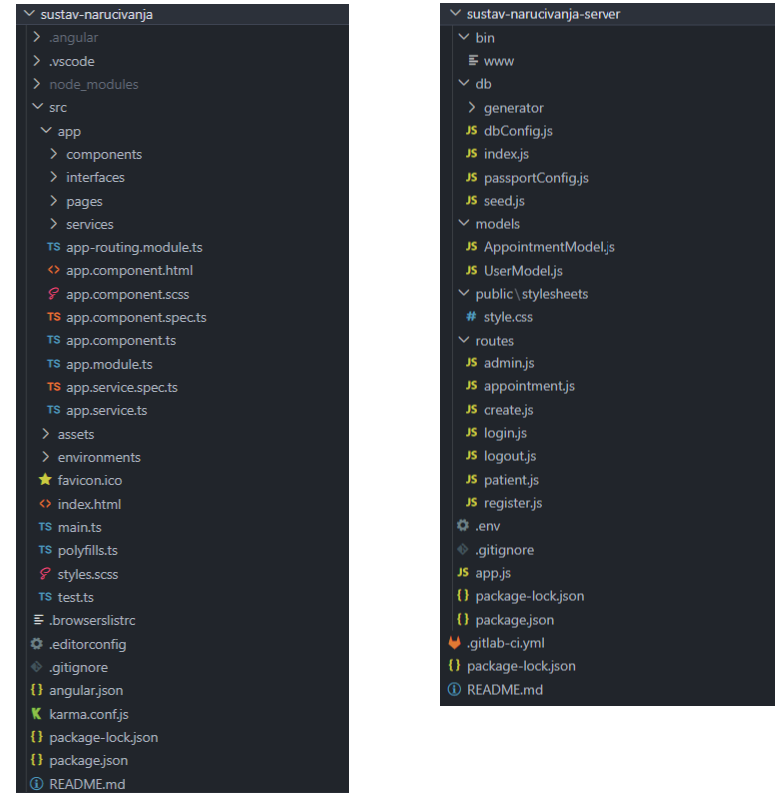
\includegraphics[width=\textwidth]{slike/struktura.png} %veličina u odnosu na širinu linije
			            \caption{Struktura implementacije aplikacije iz VSC.}
			            \label{fig:struktura} %label mora biti drugaciji za svaku sliku
		            \end{figure}

              
               \texttt{}{ Aplikaciju smo rastavili na komponente, sučelja, stranice i servise. 
               Komponente su implementirani dijelovi stranice koje možemo ubaciti kao cjelinu u neku od pages(stranica) kako ne bismo morali pisati dupli kod. Pages(stranice) su sve stranice u našoj aplikaciji. Svaki "page" sastavljen je od '.html' datoteke za strukturu, '.scss' datoteke za dizajn, '.module.ts' u kojoj možemo Typescriptom napraviti uvoz pojedinog modula Angulara u stranicu i '.ts' u kojoj definiramo putanje i povezivanje svih dokumenata.
               
               }

                \texttt{}{ Backend dio aplikacije izveden je u objektno orijentiranoj paradigmi. Pacijenti, doktori, medicinski tehničari te administratori su predstavljeni objektima koji nasljeđuju od zajedničkog roditelja, klase korisnik. Sve podklase klase korisnik znaju provjeriti svoju lozinku i korisničko ime, spremiti se u bazu te druge detalje koji su vezani za pojedinu klasu. Grupe i pregledi također su izvedeni kao klase koje sadrže metode za spremanje i dohvaćanje iz baze podataka.
               }
        
               \texttt{}{
               Razvojno okruženje koje koristite programeri Null grupe jr Visual Studio Code. Za izradu i doradu koda programeri koriste GitLab sustav.
            Za razvoj dokumentacije grupa će koristiti Overleaf aplikaciju radi sistematičnosti izrade.
               }
            
               %\includegraphics[width=\textwidth{slike/mvc.jpeg}
               
		\section{Baza podataka}
			
			\textbf{\textit{dio 1. revizije}}\\
			
		{PostgresSQL baza podataka sastoji se od 7 tablica. Entitet users je supertip koji se disjointed grana na četiri tablice: admin, patient, doctor i nurse. Primarni ključ svih tih entiteta je id koji se u tablici user automatski generira. Tablica patient također sadrži strani ključ doctorid, jer je pacijent pri registraciji obavezan izabrati svog liječnika. Tablica nurse ima strani ključ teamid, referencu na tablicu team, jer u jednom timu kojeg administrator određuje može raditi više medicinskih tehničara. Također ta vrijednost može biti null jer tehničar ne mora nužno biti dio tima. Isto vrijedi i za liječnika. Osim tih tablica također baza podataka sadrži već prije spomenutu tablicu team te appointment. Primarni ključ teama je teamid. Tablica appointment sadrži primarni ključ appointmentId koji se automatski generira te tri strana ključa. Patientid koji obavezno nije null, referenca na pacijenta koji dolazi na pregled. Druga dva strana ključa doctorId i nurseId su međusobno isključivi, odnosno ako jedan ima vrijednost, drugi mora biti null, jer pacijent dolazi na pregled ili kod liječnika ili kod tehničara. Pregled je također određen timestampom time, vremenom kad je ugovoren i intervalom duration.}
		
			\subsection{Opis tablica}
			

				%\textit{Svaku tablicu je potrebno opisati po zadanom predlošku. Lijevo se nalazi točno ime varijable u bazi podataka, u sredini se nalazi tip podataka, a desno se nalazi opis varijable. Svjetlozelenom bojom označite primarni ključ. Svjetlo plavom označite strani ključ}
				
				
				\begin{longtblr}[
					label=none,
					entry=none
					]{
						width = \textwidth,
						colspec={|X[6,l]|X[6, l]|X[20, l]|}, 
						rowhead = 1,
					} %definicija širine tablice, širine stupaca, poravnanje i broja redaka naslova tablice
					\hline \multicolumn{3}{|c|}{\textbf{users}}	 \\ \hline[3pt]
					\SetCell{LightGreen} id     &   INT     &  	Jedinstveni id svakog korisnika, generira se automatski, primarni ključ tablice korisnik \\ \hline
					name	& VARCHAR &   Ime korisnika	\\ \hline 
					surname & VARCHAR &  Prezime korisnika \\ \hline 
					 phoneNumber & VARCHAR	&  	Telefonski broj korisnika, jedinstven ta svakog korisnika	\\ \hline 
					 mail & VARCHAR	&  	Adresa elektroničke pošte korisnika, jedinstvena za svakog korisnika	\\ \hline 
					password & VARCHAR	&  	Lozinka korisnika za prijavu u sustav	\\ \hline 
					sex & VARCHAR	&  	spol korisnika	\\ \hline 
					dateOdBirth & DATE	&  	Datum rođenja korisnika	\\ \hline 
				\end{longtblr}
				
				\begin{longtblr}[
					label=none,
					entry=none
					]{
						width = \textwidth,
						colspec={|X[6,l]|X[6, l]|X[20, l]|}, 
						rowhead = 1,
					} %definicija širine tablice, širine stupaca, poravnanje i broja redaka naslova tablice
					\hline \multicolumn{3}{|c|}{\textbf{admin}}	 \\ \hline[3pt]
					\SetCell{LightGreen} id     &   INT     &  	Strani ključ, referenca na id u tablici users \\ \hline
				\end{longtblr}
				
			\begin{longtblr}[
					label=none,
					entry=none
					]{
						width = \textwidth,
						colspec={|X[12,l]|X[6, l]|X[20, l]|}, 
						rowhead = 1,
					} %definicija širine tablice, širine stupaca, poravnanje i broja redaka naslova tablice
					\hline \multicolumn{3}{|c|}{\textbf{patient}}	 \\ \hline[3pt]
					nFailedAppointments   &   INT & Broj ugovorenih pregleda koje je pacjent propustio \\ \hline
					\SetCell{LightGreen} id     &   INT     &  	Strani ključ, referenca na id u tablici users \\ \hline
					\SetCell{LightBlue} doctorid & INT & ID doktora kojeg je pacijent izabrao pri registraciji \\ \hline
				\end{longtblr}
			
			
			\begin{longtblr}[
					label=none,
					entry=none
					]{
						width = \textwidth,
						colspec={|X[6,l]|X[6, l]|X[20, l]|}, 
						rowhead = 1,
					} %definicija širine tablice, širine stupaca, poravnanje i broja redaka naslova tablice
					\hline \multicolumn{3}{|c|}{\textbf{doctor}}	 \\ \hline[3pt]
					\SetCell{LightGreen} id      &   INT     &  	Strani ključ, referenca na id u tablici users \\ \hline
					\SetCell{LightBlue}teamid & INT & Id tima kojem je doktor dodjeljen, može biti null \\\hline
				\end{longtblr}
			
			\begin{longtblr}[
					label=none,
					entry=none
					]{
						width = \textwidth,
						colspec={|X[6,l]|X[6, l]|X[20, l]|}, 
						rowhead = 1,
					} %definicija širine tablice, širine stupaca, poravnanje i broja redaka naslova tablice
					\hline \multicolumn{3}{|c|}{\textbf{nurse}}	 \\ \hline[3pt]
					\SetCell{LightGreen} id     &   INT     &  	Strani ključ, referenca na id u tablici users \\ \hline
					\SetCell{LightBlue}teamid & INT & Id tima kojem je medicinska sestra dodjeljena, može biti null \\\hline
				\end{longtblr}
				
				\begin{longtblr}[
					label=none,
					entry=none
					]{
						width = \textwidth,
						colspec={|X[6,l]|X[6, l]|X[20, l]|}, 
						rowhead = 1,
					} %definicija širine tablice, širine stupaca, poravnanje i broja redaka naslova tablice
					\hline \multicolumn{3}{|c|}{\textbf{team}}	 \\ \hline[3pt]
					\SetCell{LightGreen} teamid      &   teamid     &  	Id tima \\ \hline
				\end{longtblr}
			
			\begin{longtblr}[
					label=none,
					entry=none
					]{
						width = \textwidth,
						colspec={|X[10,l]|X[6, l]|X[20, l]|}, 
						rowhead = 1,
					} %definicija širine tablice, širine stupaca, poravnanje i broja redaka naslova tablice
					\hline \multicolumn{3}{|c|}{\textbf{appointment}}	 \\ \hline[3pt]
					\SetCell{LightGreen} id       &   INT     &  	Jedinstveni ID pregleda, generira se automatski \\ \hline
					\SetCell{LightBlue}patientid & INT & Strani ključ, ID pacijenta koji je zakazao pregled, ne može biti null \\\hline
					\SetCell{LightBlue}doctorid & INT & Strani ključ, ID doktora koji koji vrši pregled\\\hline
					\SetCell{LightBlue}nurseid & INT & Strani ključ, ID medicinskog tehničara koji vrši pregled \\\hline
					time & TIMESTAMP & Vrijeme u koje je pregled ugovoren \\ \hline
					duration & INTERVAL & Trajanje pregleda \\ \hline
				\end{longtblr}
			
			
			\subsection{Dijagram baze podataka}
				\begin{figure}[H]
			            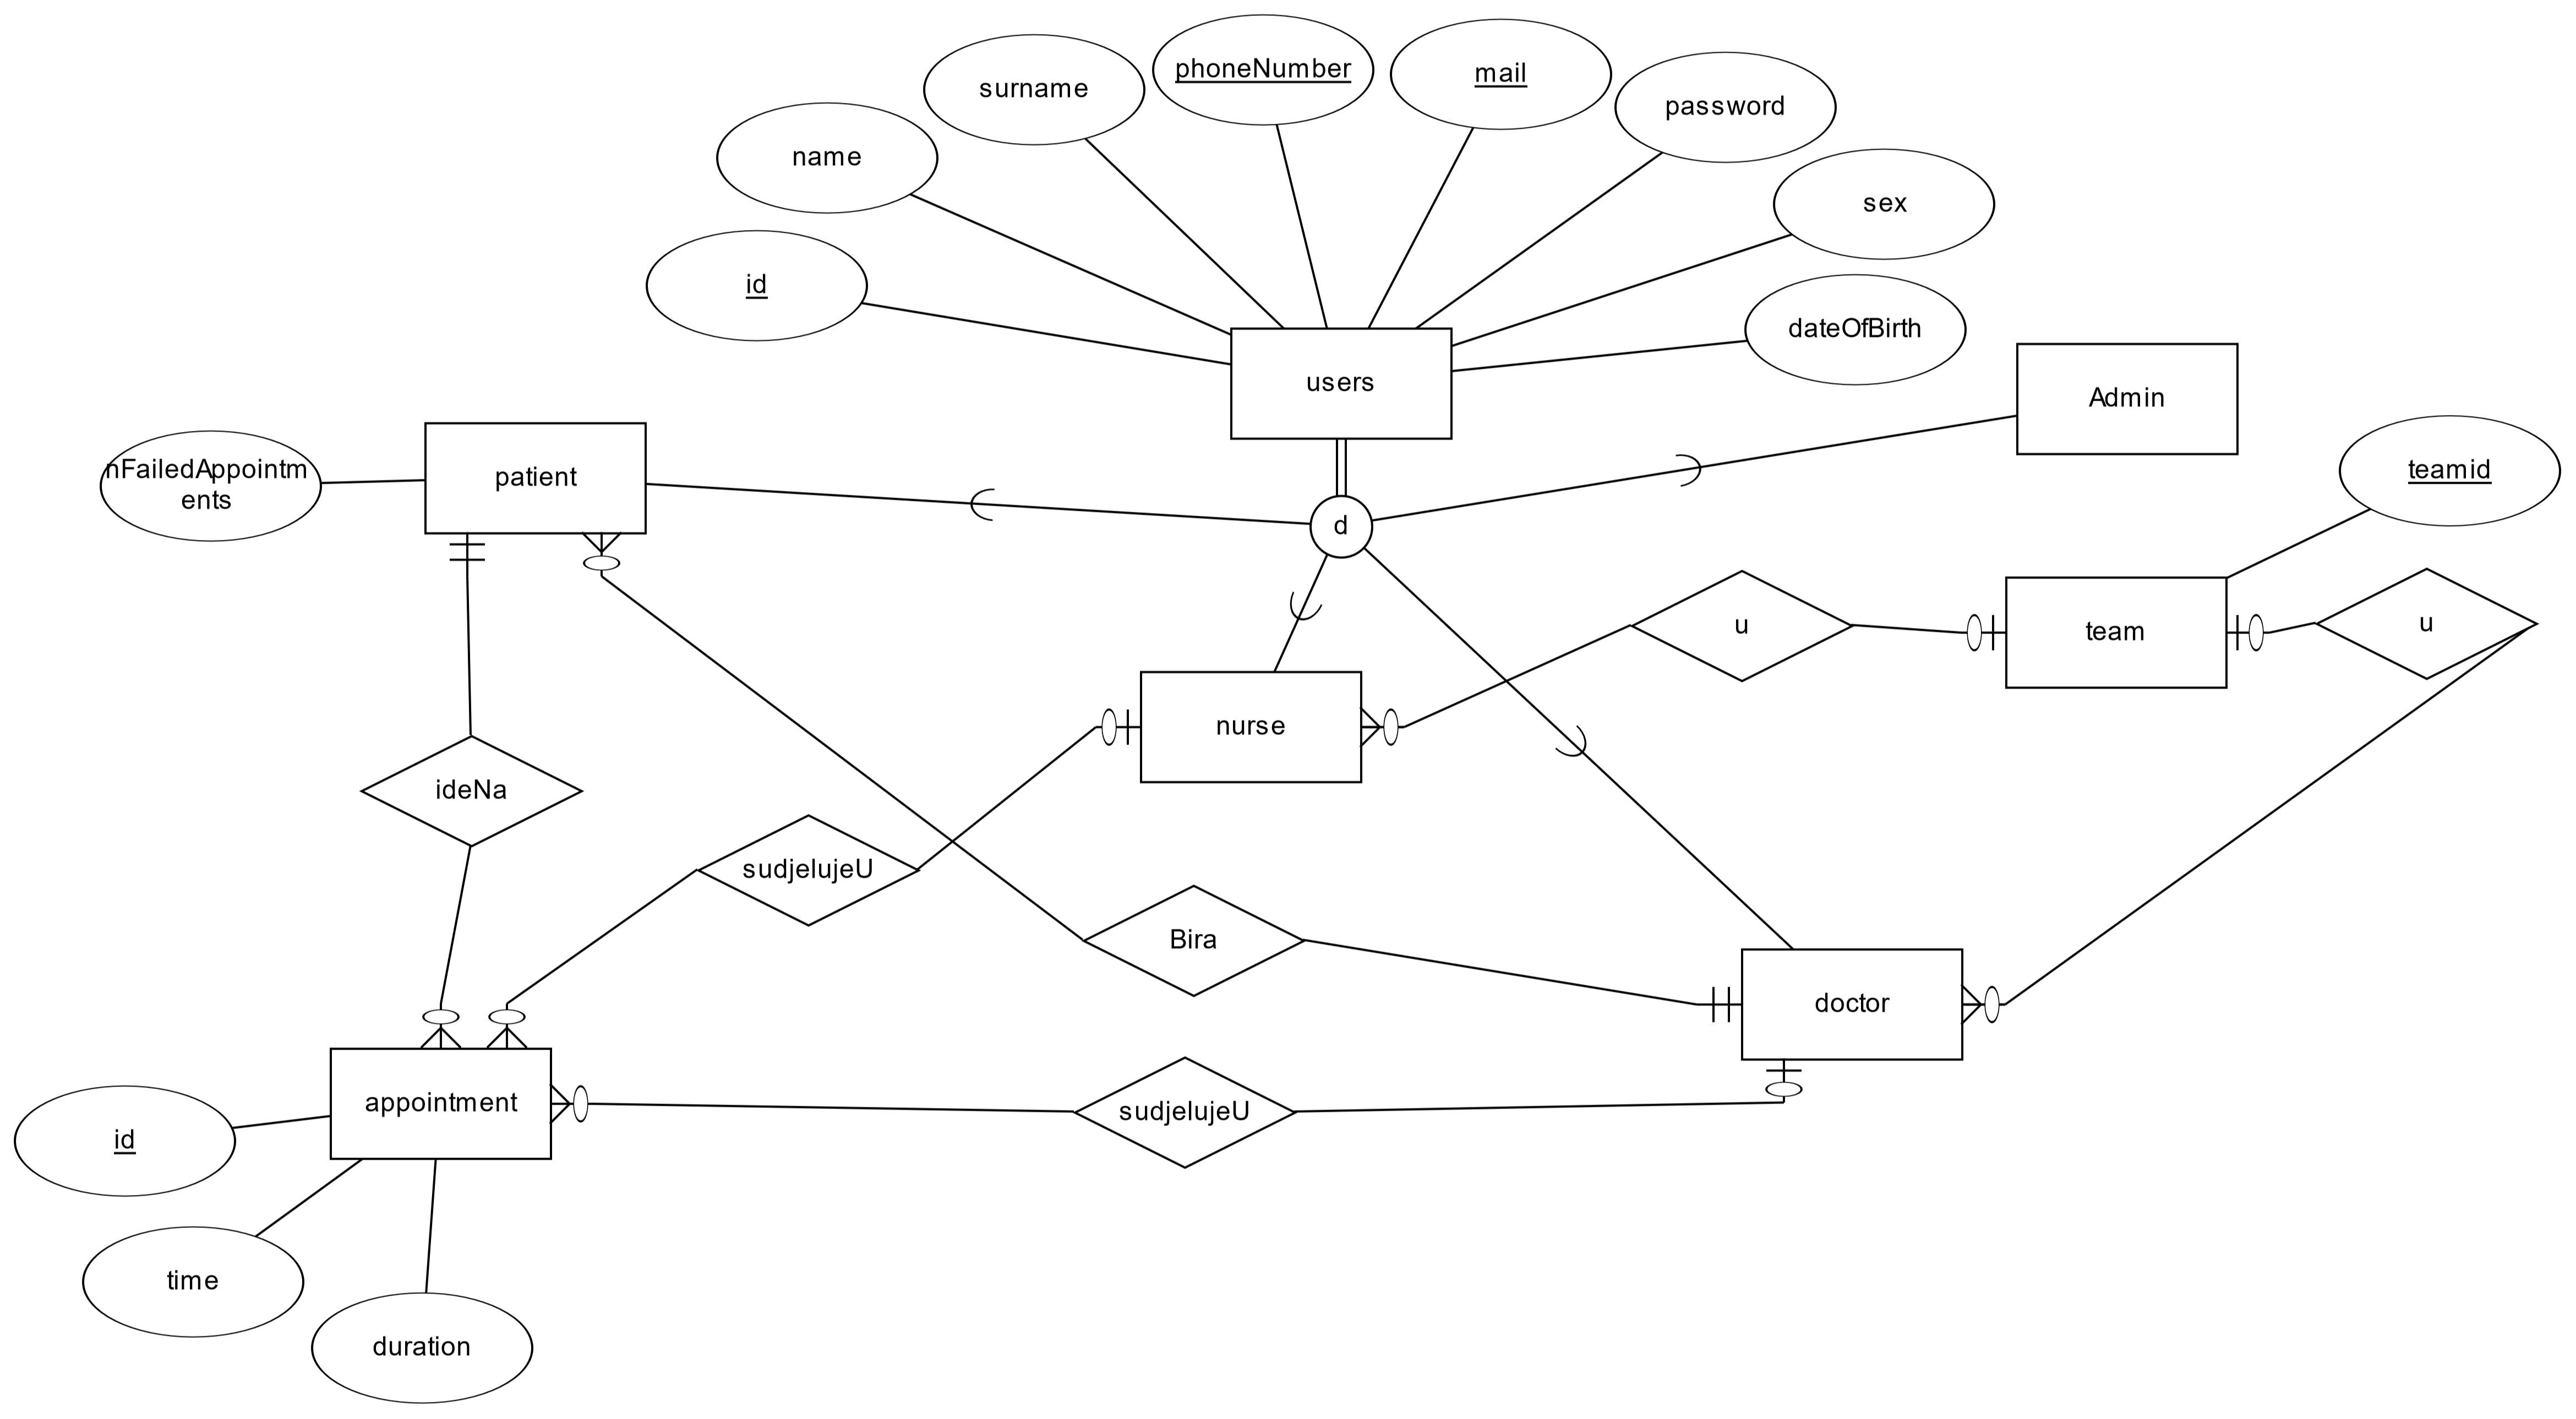
\includegraphics[width=\textwidth]{slike/erplus.png} %veličina u odnosu na širinu linije
			            \caption{ER dijagram baze podataka}
			            \label{fig:bp1} %label mora biti drugaciji za svaku sliku
		            \end{figure}			
			\subsection{Dijagram baze podataka}
				\begin{figure}[H]
			            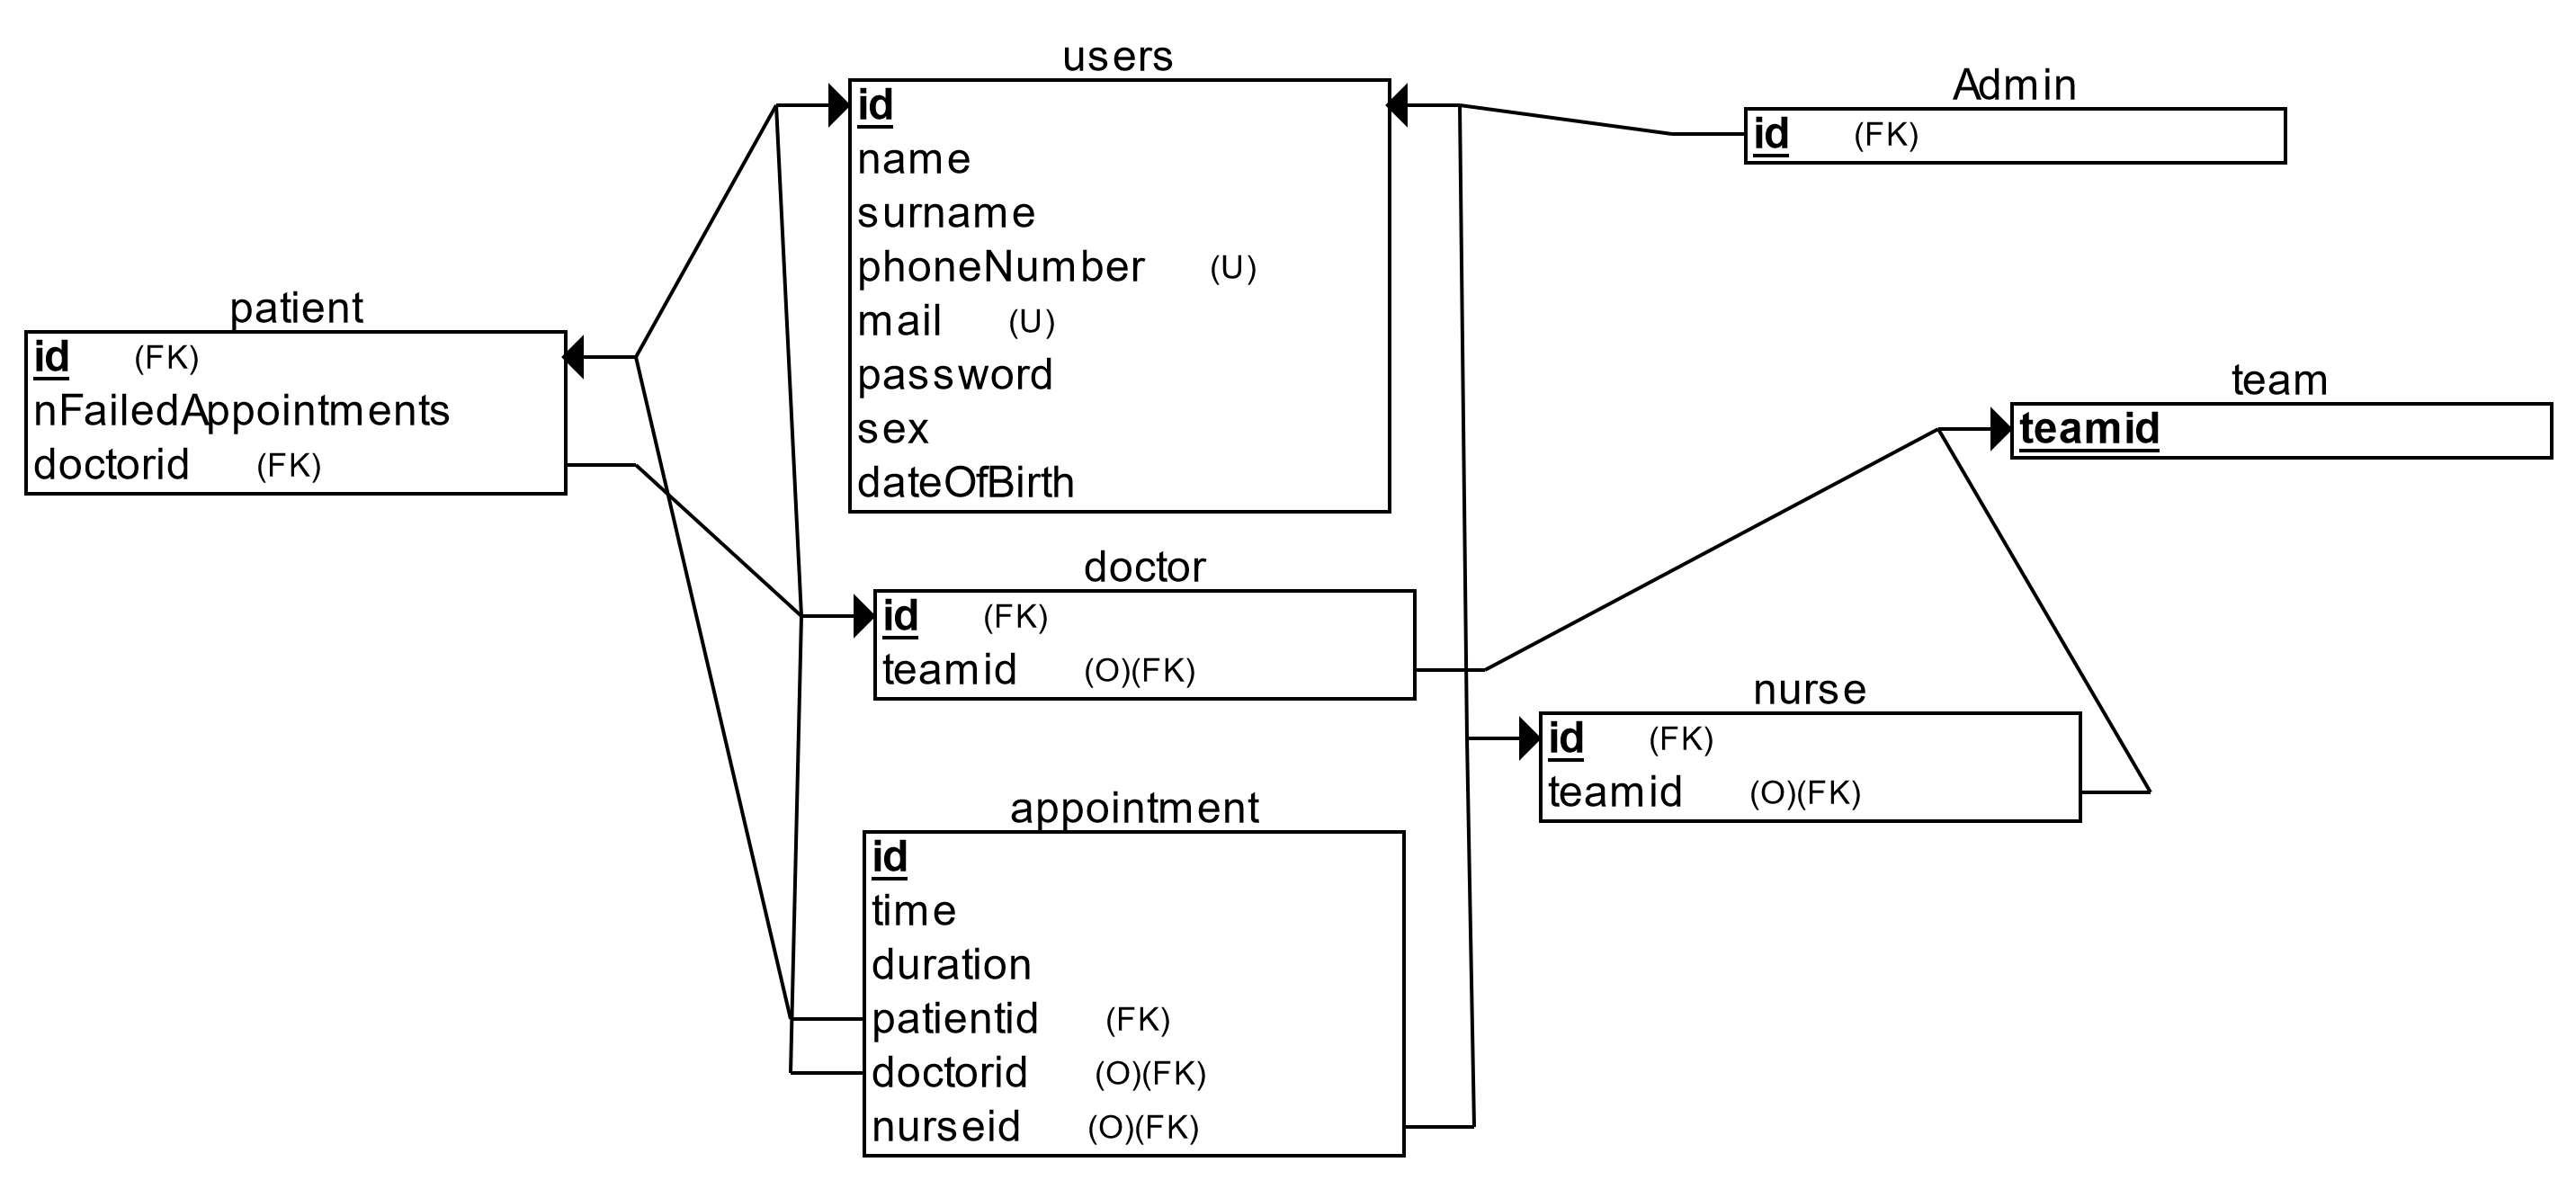
\includegraphics[width=\textwidth]{slike/relacijski.png} %veličina u odnosu na širinu linije
			            \caption{Relacijski dijagram baze podataka}
			            \label{fig:bp2} %label mora biti drugaciji za svaku sliku
		            \end{figure}
		            
			
			\eject
			
			
		\section{Dijagram razreda}
		
			%\textit{Potrebno je priložiti dijagram razreda s pripadajućim opisom. Zbog preglednosti je moguće dijagram razlomiti na više njih, ali moraju biti grupirani prema sličnim razinama apstrakcije i srodnim funkcionalnostima.}\\
			
			%\textbf{\textit{dio 1. revizije}}\\
			
			%\textit{Prilikom prve predaje projekta, potrebno je priložiti potpuno razrađen dijagram razreda vezan uz \textbf{generičku funkcionalnost} sustava. Ostale funkcionalnosti trebaju biti idejno razrađene u dijagramu sa sljedećim komponentama: nazivi razreda, nazivi metoda i vrste pristupa metodama (npr. javni, zaštićeni), nazivi atributa razreda, veze i odnosi između razreda.}\\
			
			Na slici 4.4 prikazan je dijagram razreda koji pripada backend dijelu arhitekture. Razredi iz dijagrama predstavljaju strukturu baze podataka u aplikaciji te svaki razred predstavlja jedan entitet iz baze. Metode koje su implementirane komuniciraju s bazom podataka, ako je potrebno, upisuju odgovarajuće podatke u bazu ili ih vraćaju iz baze. Razred User predstavlja svakog korisnika aplikacije i koji može koristiti određene funkcionalnosti sustava. Međutim, prije toga se mora registrirati s osobnim podacima: ime, prezime, spol, broj telefona, e-mail, lozinka i datum rođenja. Razred Pacijent predstavlja korisnika koji je registriran kao pacijent i ima pristup svojim terminima uz funkcionalnosti zakazivanja i otkazivanja termina, kojeg predstavlja razred Appointment. Nešto veću ovlast ima medicinska sestra koju predstavlja razred Nurse, ona može i unaprijed definirati termine usluga. Razred Doctor predstavlja liječnika koji može definirati slobodne termine pregleda, ali i definirati pravila za naručivanje. Najvišu ovlast ima administrator, kojeg predstavlja razred Admin. On može stvarati timove, koje predstavlja razred Teams, te upisati nove liječnike i medicinske sestre u bazu.
			
			\begin{figure}[H]
			            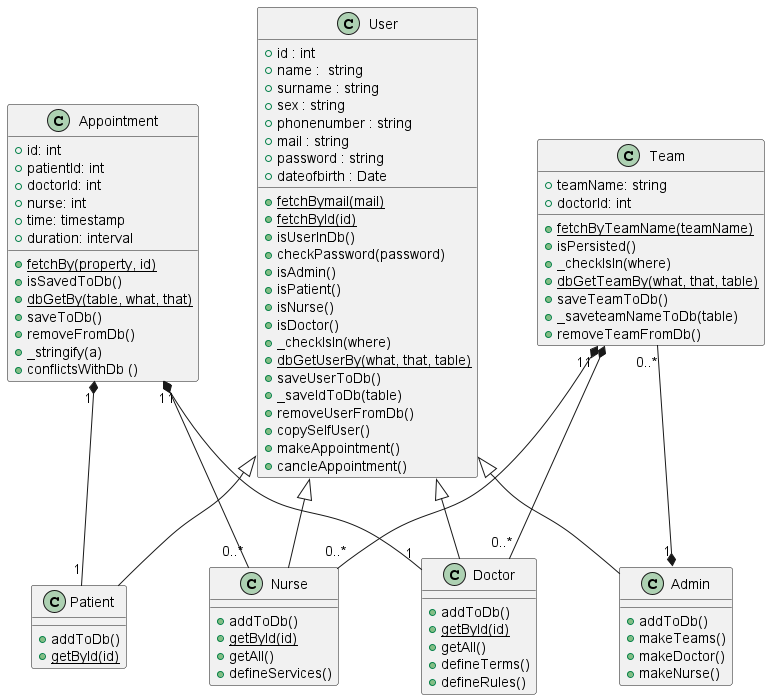
\includegraphics[width=\textwidth]{slike/backend_class_diagram.png} %veličina u odnosu na širinu linije
			            \caption{Dijagram razreda - Modeli}
			            \label{fig:class1} %label mora biti drugaciji za svaku sliku
		      \end{figure}
		      
		      \eject
		      
		      
		        Dijagram razreda na slici 4.5 generirali smo pomoću 'Classdiagram -ts' ekstenzije autora Alexa Shena u razvojnom okruženju Visual Studio Code. Dijagram prikazuje strukturu frontend dijela aplikacije. Angular je framework koji se bazira na komponentama, te svaka komponenta, koja je osnovni i gradivni dio, koristi neki od modula koji ih povezuju. Tako korijenski modul aplikacije, AppRoutingModule koristi svi nadređene module kao što su HomeModule, TeamModule, AdminModule, PatientModule, TechModule i DoctorModule, a svaka od njih koriste MainFooterModule i MainNavigationModule. Korištenjem komponenata smanjujemo redundanciju u kodu. Ovisno o tome koje ovlasti ima, bio on doktor, medicinska sestra pacijent ili administator, korisniku su prikazane različite komponente. Na primjer, pacijent ima pristup komponentama: KalendarComponent, MainNavigationComponent i MainFooterComponet.Za svaku komponentu korisniku su prikazani njihovi html predlošci, css oblikovanja i funkcionlanosti definirane u pojedinom dijelu komponente.
                 
		      
		   \begin{figure}[H]
			            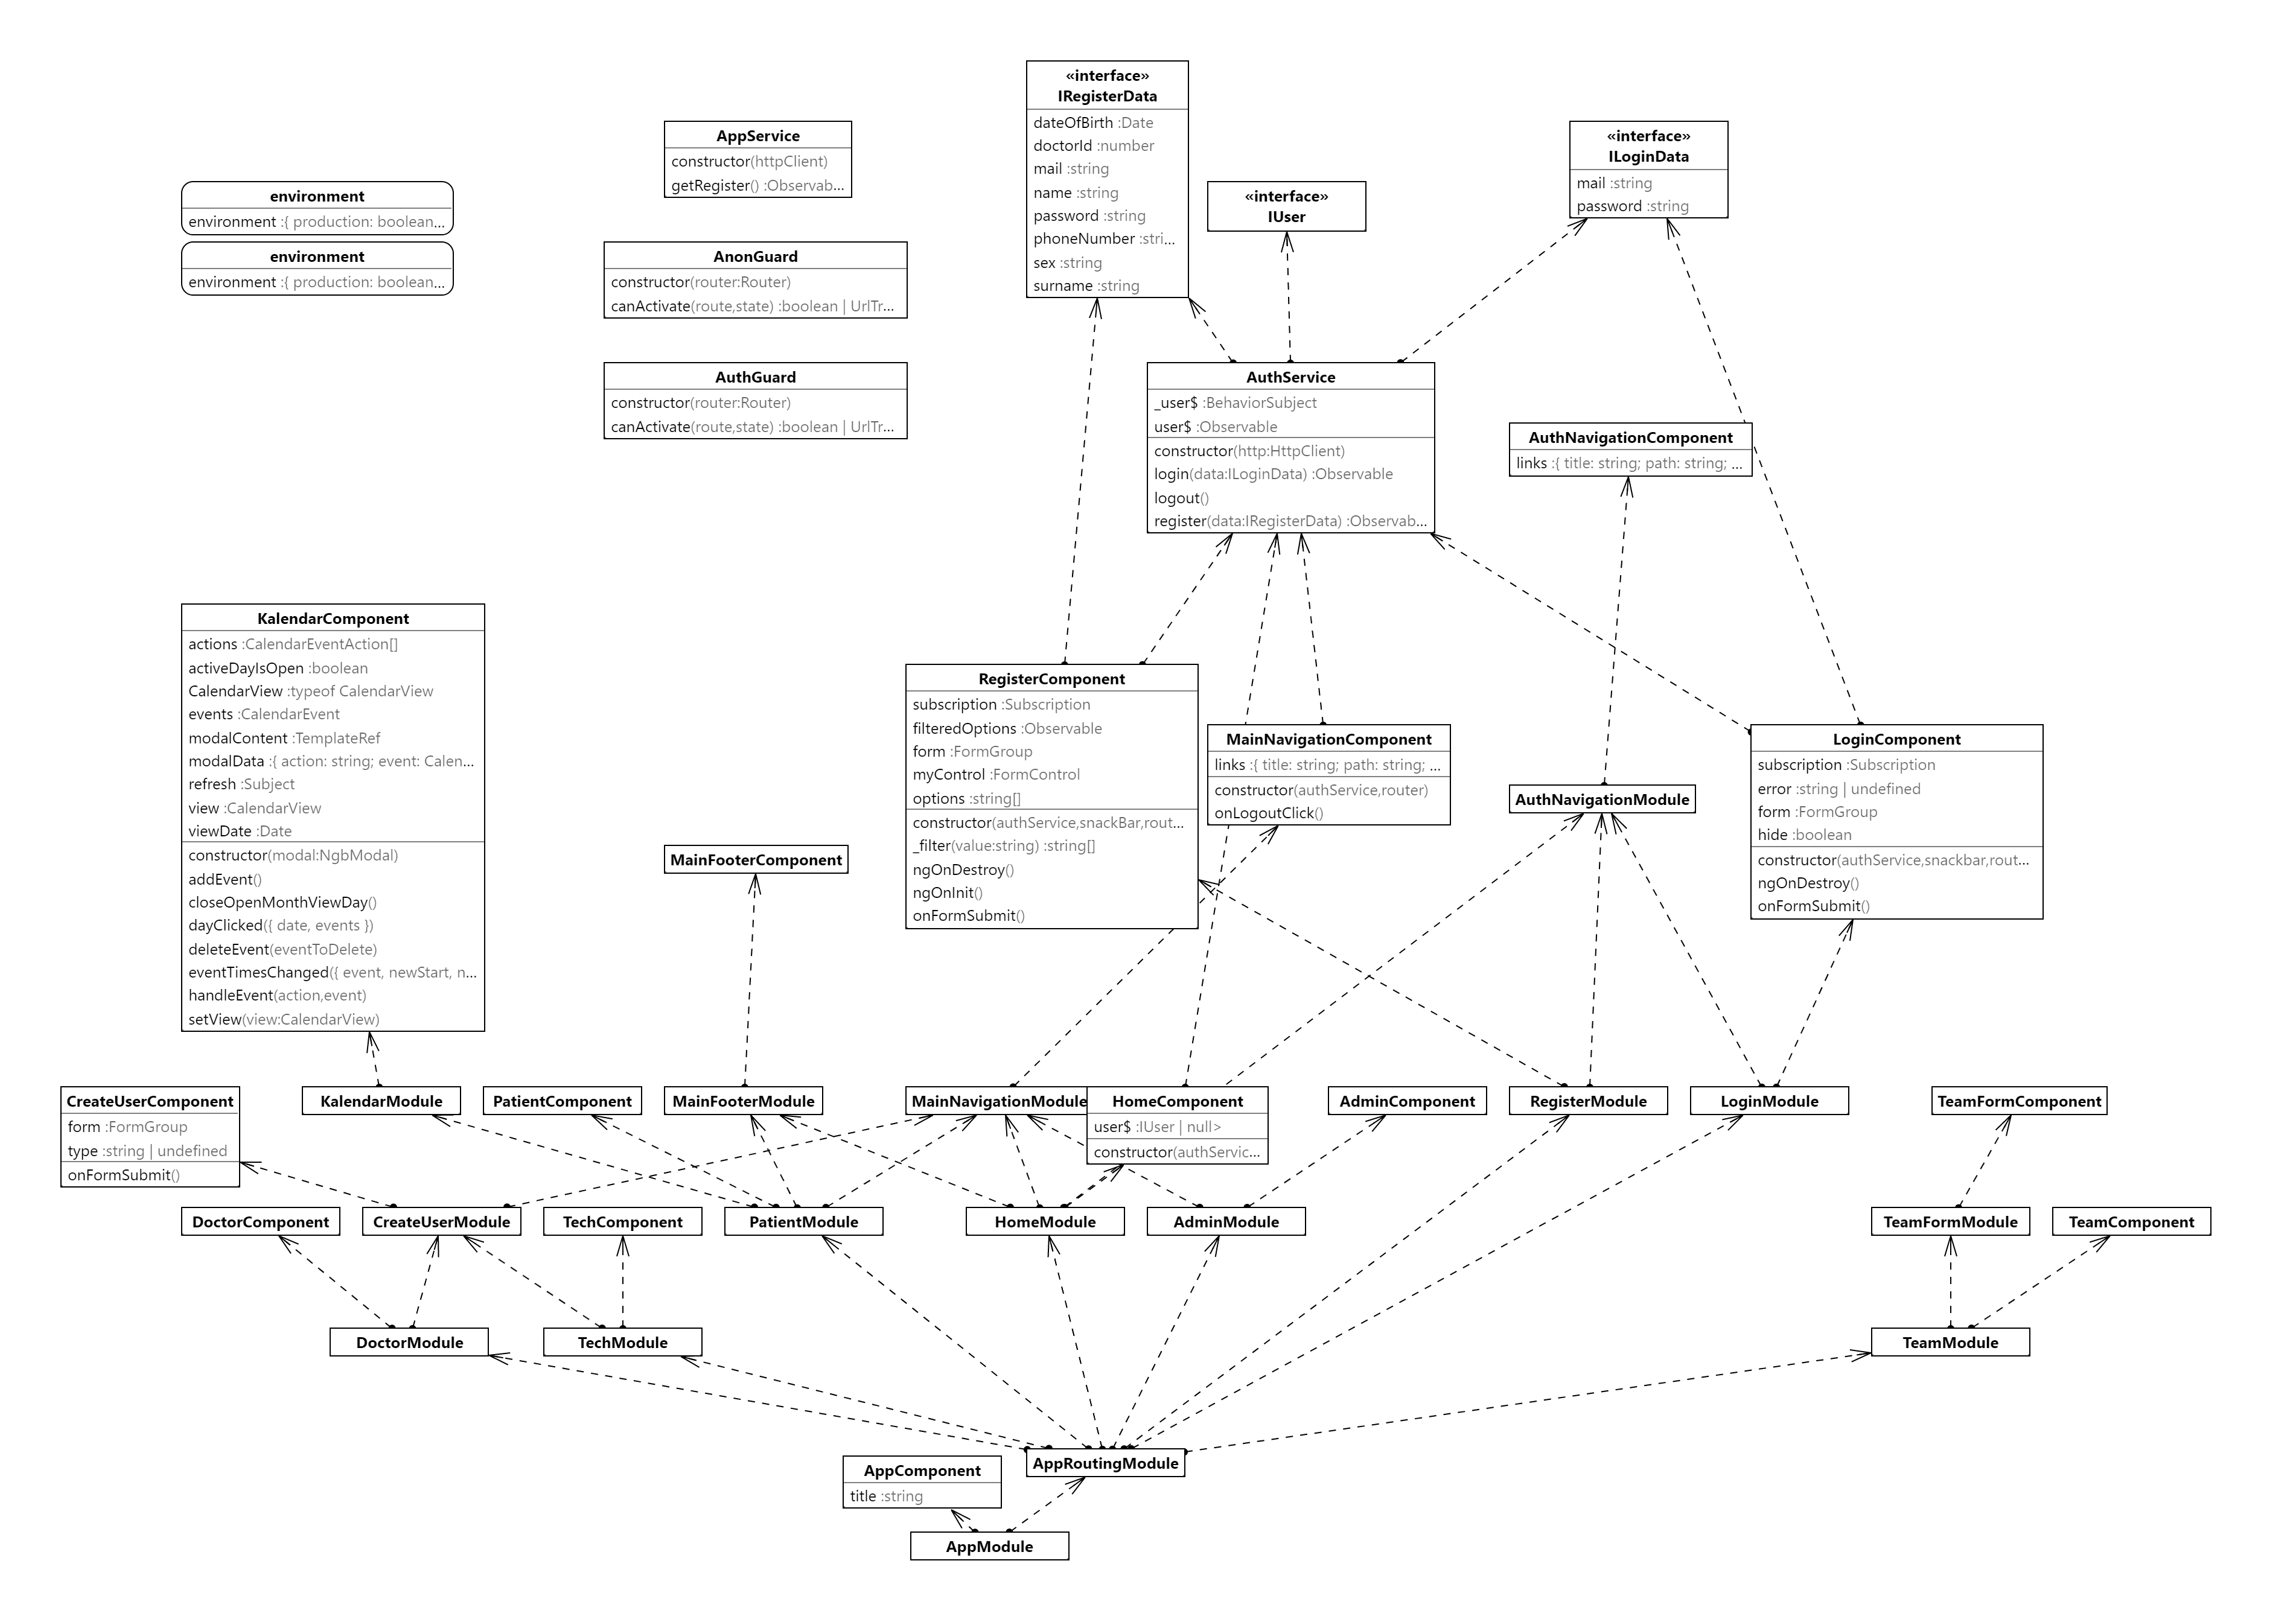
\includegraphics[width=\textwidth]{slike/frontend_class_diagram.png} %veličina u odnosu na širinu linije
			          \caption{Dijagram razreda - frontend}
			            \label{fig:class2} %label mora biti drugaciji za svaku sliku
		      \end{figure}
                 
                
			
		%	\textbf{\textit{dio 2. revizije}}\\			
			
		%	\textit{Prilikom druge predaje projekta dijagram razreda i opisi moraju odgovarati stvarnom stanju implementacije}
			
			
			
		%	\eject
		
		%\section{Dijagram stanja}
			
			
			%\textbf{\textit{dio 2. revizije}}\\
			
			%\textit{Potrebno je priložiti dijagram stanja i opisati ga. Dovoljan je jedan dijagram stanja koji prikazuje \textbf{značajan dio funkcionalnosti} sustava. Na primjer, stanja korisničkog sučelja i tijek korištenja neke ključne funkcionalnosti jesu značajan dio sustava, a registracija i prijava nisu. }
			
			
			%\eject 
		
		%\section{Dijagram aktivnosti}
			
			%\textbf{\textit{dio 2. revizije}}\\
			
			 %\textit{Potrebno je priložiti dijagram aktivnosti s pripadajućim opisom. Dijagram aktivnosti treba prikazivati značajan dio sustava.}
			
			%\eject
		%\section{Dijagram komponenti}
		
			%\textbf{\textit{dio 2. revizije}}\\
		
			 %\textit{Potrebno je priložiti dijagram komponenti s pripadajućim opisom. Dijagram komponenti treba prikazivati strukturu cijele aplikacije.}
	\chapter{Implementacija i korisničko sučelje}
		
		
		\section{Korištene tehnologije i alati}
		
			\textbf{\textit{dio 2. revizije}}
			
			 \textit{Detaljno navesti sve tehnologije i alate koji su primijenjeni pri izradi dokumentacije i aplikacije. Ukratko ih opisati, te navesti njihovo značenje i mjesto primjene. Za svaki navedeni alat i tehnologiju je potrebno \textbf{navesti internet poveznicu} gdje se mogu preuzeti ili više saznati o njima}.
			
			
			\eject 
		
	
		\section{Ispitivanje programskog rješenja}
	
			
			\subsection{Ispitivanje komponenti}
			\textit{Ispitivanje komponenti ostvareno je korištenjem Jest alata za ispi-
                    tivanje. U nastavku su opisani provedeni testovi te priložene funkcija za tesriranje te izlaz koji se dobije testiranjem. Prikazani testovi pokrivaju klase UserModel i AppointmentModel koje implementiraju najvažnije funkcionalnosti aplikacije
                    }

            \begin{figure}[H]
                    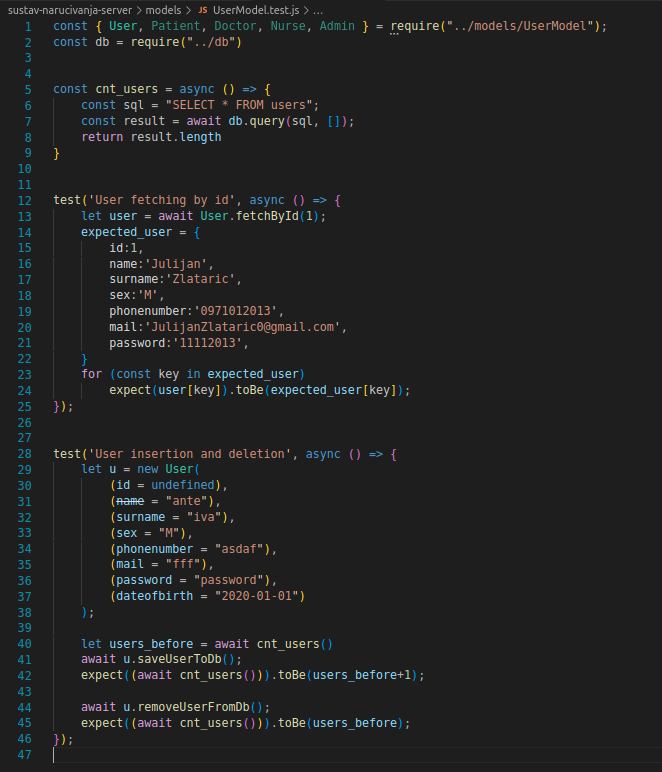
\includegraphics[width=300]{slike/usermodel_tests_code.png} %veličina u odnosu na širinu linije
                    \caption{Prikazani testovi testiraju dohvachanje usera iz baze podataka te njegovo ubacivanje i izbacivanje iz baze podataka. Navedene funkcionalnosti su nuzhne za pravilnu registraciju i login korisnika aplikacije.}
                    \label{fig:struktura} %label mora biti drugaciji za svaku sliku
                \end{figure}

                \begin{figure}[H]
                    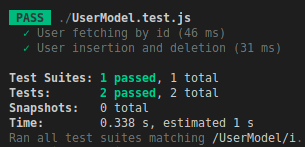
\includegraphics[width=\textwidth]{slike/usermodel_tests_out.png} %veličina u odnosu na širinu linije
                    \caption{Izlaz programa za testiranje klase UserModel s 2 testna primjera. Sa slike je vidljivo da klasa prolazi testne primjere.}
                    \label{fig:struktura} %label mora biti drugaciji za svaku sliku
                \end{figure}

            \begin{figure}[H]
                    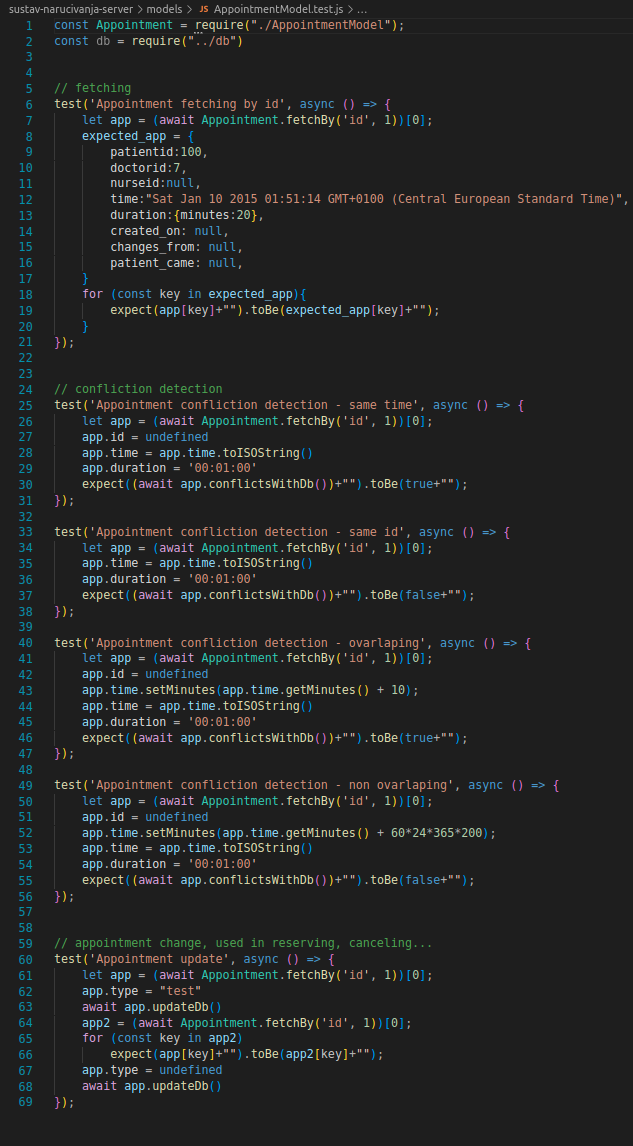
\includegraphics[width=300]{slike/appointment_tests_code.png} %veličina u odnosu na širinu linije
                    \caption{Prikazani testovi testiraju dohvachanje odredzenog termina iz baze podataka, testiranje postoji li odredzeni termin koji je u vremenskom konfliktu s odabranim terminom te testiranje updateanja termina. Testiranje konflikata ima vise rubnih sluchajeva, naime isti termin mogli smo vecz dohvatiti iz baze podataka te tada nebi trebalo biti konflikata, zatim mogucze je da se termin nalazi unutar drugoga, potpuno izvan...}
                    \label{fig:struktura} %label mora biti drugaciji za svaku sliku
                \end{figure}

                \begin{figure}[H]
                    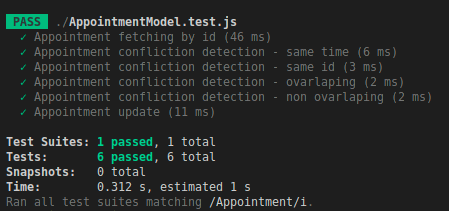
\includegraphics[width=\textwidth]{slike/appointment_tests_out.png} %veličina u odnosu na širinu linije
                    \caption{Izlaz programa za testiranje klase AppointmentModel s 6 testnih primjera. Sa slike je vidljivo da klasa prolazi testne primjere.}
                    \label{fig:struktura} %label mora biti drugaciji za svaku sliku
                \end{figure}
			
			
			
			\subsection{Ispitivanje sustava}
			
			 \textit{Potrebno je provesti i opisati ispitivanje sustava koristeći radni okvir Selenium\footnote{\url{https://www.seleniumhq.org/}}. Razraditi \textbf{minimalno 4 ispitna slučaja} u kojima će se ispitati redovni slučajevi, rubni uvjeti te poziv funkcionalnosti koja nije implementirana/izaziva pogrešku kako bi se vidjelo na koji način sustav reagira kada nešto nije u potpunosti ostvareno. Ispitni slučaj se treba sastojati od ulaza (npr. korisničko ime i lozinka), očekivanog izlaza ili rezultata, koraka ispitivanja i dobivenog izlaza ili rezultata.\\ }
			 
			 \textit{Izradu ispitnih slučajeva pomoću radnog okvira Selenium moguće je provesti pomoću jednog od sljedeća dva alata:}
			 \begin{itemize}
			 	\item \textit{dodatak za preglednik \textbf{Selenium IDE} - snimanje korisnikovih akcija radi automatskog ponavljanja ispita	}
			 	\item \textit{\textbf{Selenium WebDriver} - podrška za pisanje ispita u jezicima Java, C\#, PHP koristeći posebno programsko sučelje.}
			 \end{itemize}
		 	\textit{Detalji o korištenju alata Selenium bit će prikazani na posebnom predavanju tijekom semestra.}
			
			\eject 

           \begin{figure}[H]
                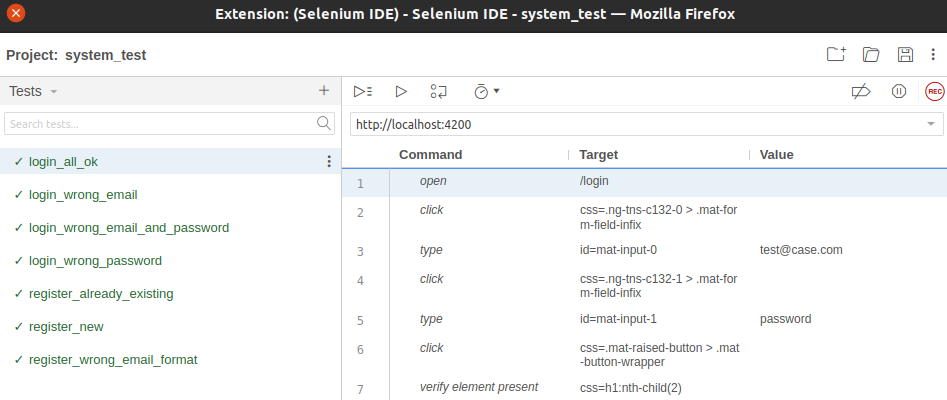
\includegraphics[width=\textwidth]{slike/tests_system/login_all_ok.png} %veličina u odnosu na širinu linije
                \caption{Program za testiranje.}
                \label{fig:struktura} %label mora biti drugaciji za svaku sliku
            \end{figure}

            \begin{figure}[H]
                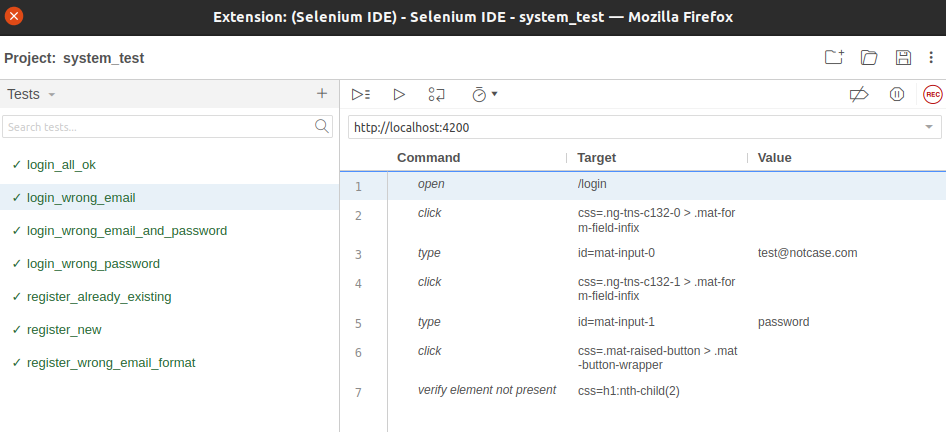
\includegraphics[width=\textwidth]{slike/tests_system/login_wrong_email.png} %veličina u odnosu na širinu linije
                \caption{Program za testiranje.}
                \label{fig:struktura} %label mora biti drugaciji za svaku sliku
            \end{figure}

            \begin{figure}[H]
                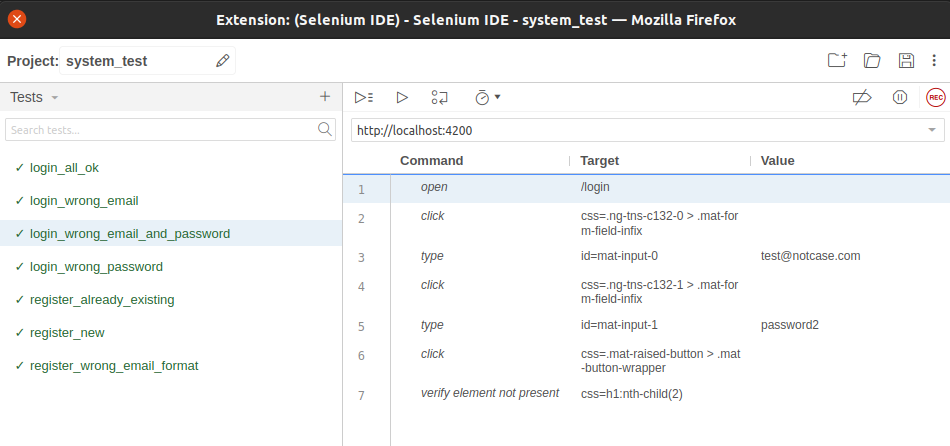
\includegraphics[width=\textwidth]{slike/tests_system/login_wrong_email_and_password.png} %veličina u odnosu na širinu linije
                \caption{Program za testiranje.}
                \label{fig:struktura} %label mora biti drugaciji za svaku sliku
            \end{figure}

            \begin{figure}[H]
                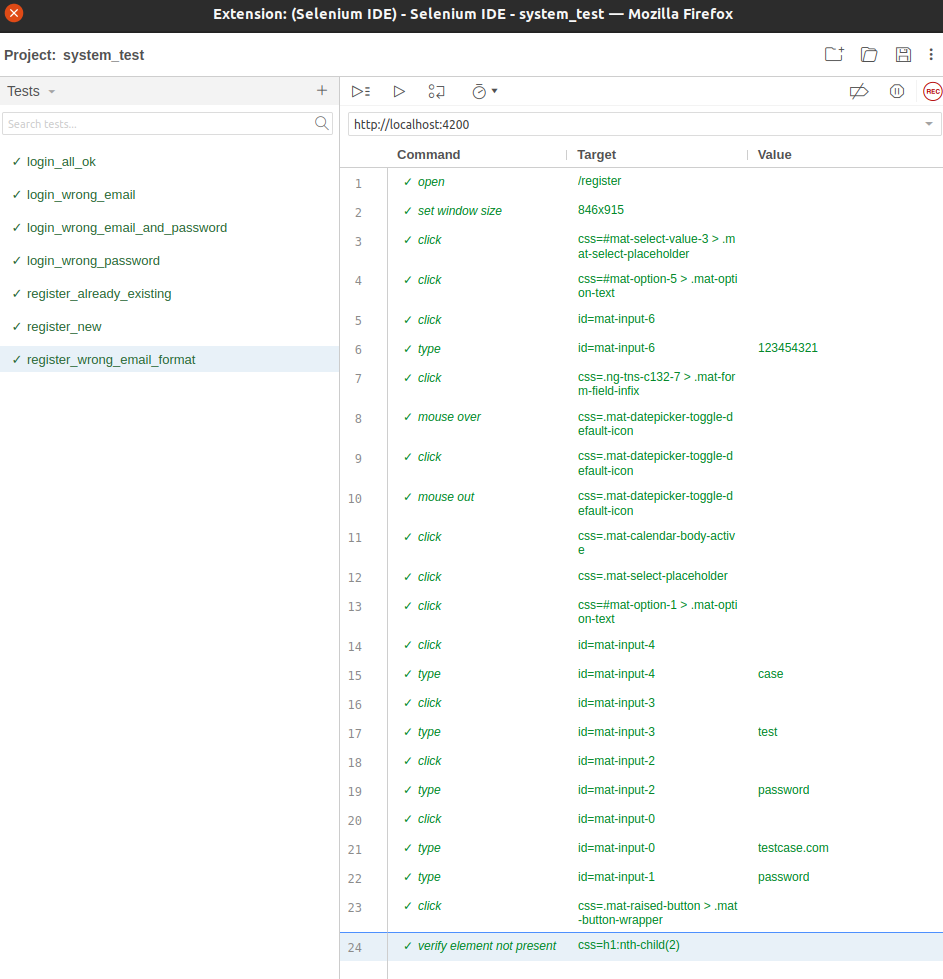
\includegraphics[width=\textwidth]{slike/tests_system/register_wrong_format.png} %veličina u odnosu na širinu linije
                \caption{Program za testiranje.}
                \label{fig:struktura} %label mora biti drugaciji za svaku sliku
            \end{figure}

            \begin{figure}[H]
                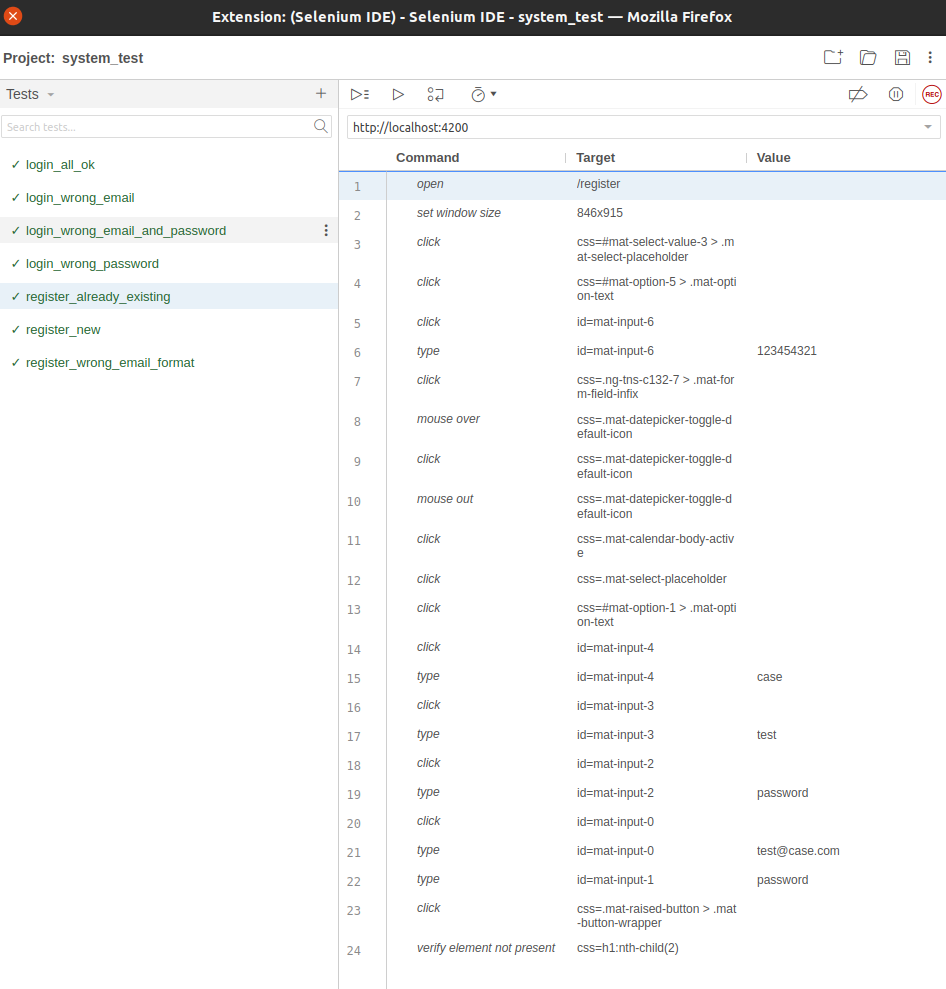
\includegraphics[width=\textwidth]{slike/tests_system/register_already_existing.png} %veličina u odnosu na širinu linije
                \caption{Program za testiranje.}
                \label{fig:struktura} %label mora biti drugaciji za svaku sliku
            \end{figure}

            \begin{figure}[H]
                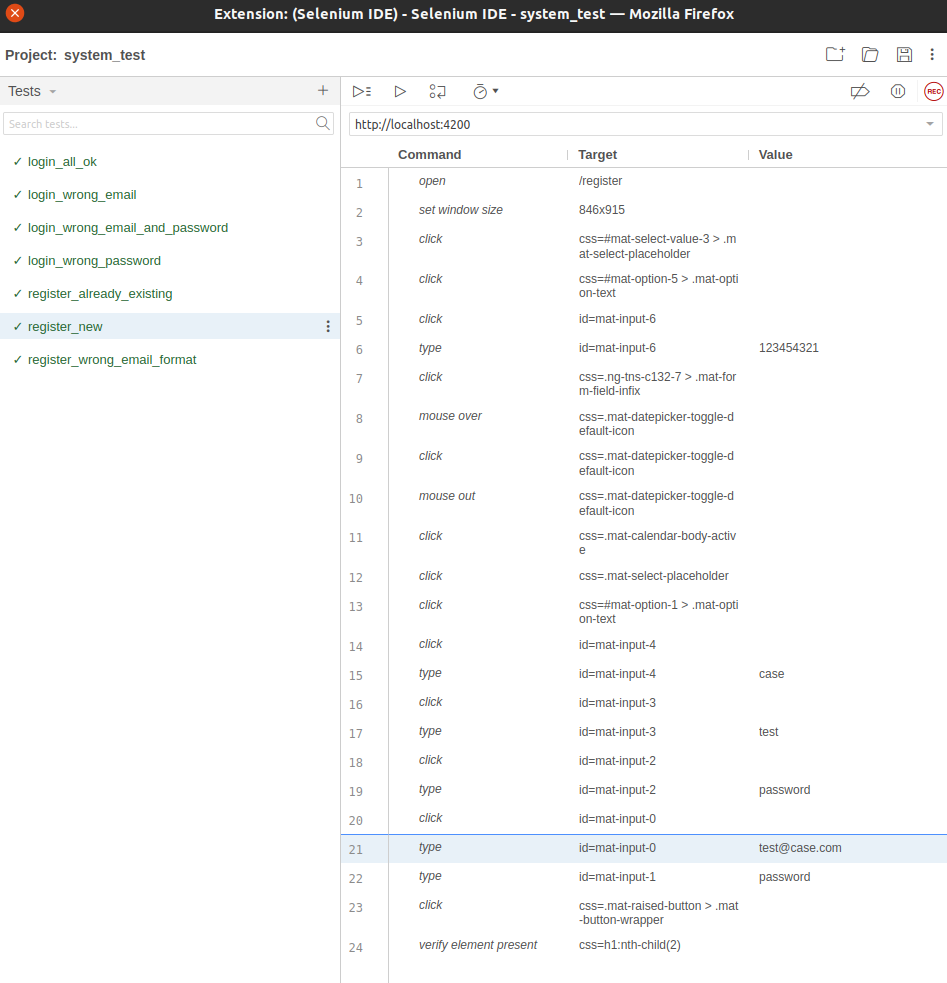
\includegraphics[width=\textwidth]{slike/tests_system/register_new.png} %veličina u odnosu na širinu linije
                \caption{Program za testiranje.}
                \label{fig:struktura} %label mora biti drugaciji za svaku sliku
            \end{figure}
		
		\section{Dijagram razmještaja}
			
			\textbf{\textit{dio 2. revizije}}
			
			 \textit{Potrebno je umetnuti \textbf{specifikacijski} dijagram razmještaja i opisati ga. Moguće je umjesto specifikacijskog dijagrama razmještaja umetnuti dijagram razmještaja instanci, pod uvjetom da taj dijagram bolje opisuje neki važniji dio sustava.}
			
			\eject 
		
		\section{Upute za puštanje u pogon}
		
			\textbf{\textit{dio 2. revizije}}\\
		
			 \textit{U ovom poglavlju potrebno je dati upute za puštanje u pogon (engl. deployment) ostvarene aplikacije. Na primjer, za web aplikacije, opisati postupak kojim se od izvornog kôda dolazi do potpuno postavljene baze podataka i poslužitelja koji odgovara na upite korisnika. Za mobilnu aplikaciju, postupak kojim se aplikacija izgradi, te postavi na neku od trgovina. Za stolnu (engl. desktop) aplikaciju, postupak kojim se aplikacija instalira na računalo. Ukoliko mobilne i stolne aplikacije komuniciraju s poslužiteljem i/ili bazom podataka, opisati i postupak njihovog postavljanja. Pri izradi uputa preporučuje se \textbf{naglasiti korake instalacije uporabom natuknica} te koristiti što je više moguće \textbf{slike ekrana} (engl. screenshots) kako bi upute bile jasne i jednostavne za slijediti.}
			
			
			 \textit{Dovršenu aplikaciju potrebno je pokrenuti na javno dostupnom poslužitelju. Studentima se preporuča korištenje neke od sljedećih besplatnih usluga: \href{https://aws.amazon.com/}{Amazon AWS}, \href{https://azure.microsoft.com/en-us/}{Microsoft Azure} ili \href{https://www.heroku.com/}{Heroku}. Mobilne aplikacije trebaju biti objavljene na F-Droid, Google Play ili Amazon App trgovini.}
			
			
			\eject 
	\chapter{Zaključak}
		
		 \texttt{}{Zadatak naše grupe bila je implementacija sustava za naručivanje pregleda u hrvatskom zdravstvu. Kroz našu aplikaciju pacijenti mogu zakazivati termine ovisno o dostupnosti pojedinih doktora/medicinskih radnika. Nakon 14 tjedana rada, naša grupa je ostvarila upotebljivu aplikaciju koja ispunjava sve korisničke zahtjeve koji su bili zadani za nju. }
   
   
          \texttt{}{
          Prvi ciklus izrade projekta zahtjevao je okupljanje tima. Nakon okupljanja, prva podjela tima bila je na frontend i backend domenu. Darijan Gudelj, Branimir Tomeljak i Vilim Ivanković preuzeli su backend domenu, a Luka Slugečić, Bruno Rački i Marin Teskera preuzeli su frontend domenu. Kako je frontend domena bila ograničena poslom, neki članovi frontend domene pomagali su pri izradi backend domene. Nakon izrade prvostupničke aplikacije koja je funkcionirala u minornim zahtjevima, naša grupa je krenula na izradu dokumentacije. Izradili smo sekvencijske dijagrame, obrasce upotrebe, dijagram razreda i model baze podataka. Svi ti modeli olakšali su razumijevanje i izradu novih komponenti u drugom ciklusu rada. Sastanci su se održavali barem jednom na tjednoj bazi, te su članovi NULL grupe ulagali jako puno samostalnog truda i rada između sastanaka.
          }

          \texttt{}{
          Drugi ciklus izrade projekta zahjtevao je da se domene razmijenjuju, tako se većina timova prebacivala po potrebi u drugu domenu. Kako je posla bilo previše, NULL grupa sastajala se dva puta tjedno kako bi uspješno izvršila sve korisničke zahtjeve. U drugom ciklusu radili smo na implementaciji aplikacije koja posjeduje autentifikaciju, nema nepredvidive greške i točno su određene mogućnosti pojedinog korisnika u aplikaciji. Implementirali smo izvješća, SMS poruke, emailove, kalendar itd.. Kako je posao rastao i postajao sve kompleksnije NULL grupa komunicirala je dvjema kanalima, a to su Discord i Whatsapp koji su nam uvelike pomogli u rješavanju problema. Svakodnevno smo komunicirali i izmijenjivali iskustva u izradi ovoga sustava i to sa vjerodostojnošću radili. Nakon završene aplikacije izradili smo i dijagram aktivnosti, stanja i komponenti. 

          Mogućnost izrade ovog projekta svakome članu NULL grupe dala je nova programska i komunikativna iskustva koje nikada nećemo zaboraviti. Svaki član osjetio je koliko je bitno znati raditi u timu i koliko je svačiji rad blagonosan. Kao tim smo se uspjeli organizirati, slušali smo jedni druge i ono što je najbitnije, učili jedni od drugih. 

          Svaki član je zadovoljan postignutim i trudit ćemo se u budućnosti koristiti znanje dobiveno na ovome projektu.
          }
		
		\eject 
	\chapter*{Popis literature}
		\addcontentsline{toc}{chapter}{Popis literature}
	 	
 		\textbf{\textit{Kontinuirano osvježavanje}}
	
		%\textit{Popisati sve reference i literaturu koja je pomogla pri ostvarivanju projekta.}
		
		
		\begin{enumerate}
			
			
			\item  Programsko inženjerstvo, FER ZEMRIS, \url{https://www.fer.unizg.hr/predmet/proinz}
			
			\item  I. Sommerville, "Software engineering", 8th ed, Addison Wesley, 2007.
			
			\item  T.C.Lethbridge, R.Langaniere, "Object-Oriented Software Engineering", 2nd ed. McGraw-Hill, 2005.
			
			\item  I. Marsic, Software engineering book``, Department of Electrical and Computer Engineering, Rutgers University, \url{http://www.ece.rutgers.edu/~marsic/books/SE}
			
			\item  The Unified Modeling Language, \url{https://www.uml-diagrams.org/}
			
			\item  Astah Community, \url{http://astah.net/editions/uml-new}
		\end{enumerate}
		
		 
	
	
	\begingroup
	\renewcommand*\listfigurename{Indeks slika i dijagrama}
	%\renewcommand*\listtablename{Indeks tablica}
	%\let\clearpage\relax
	\listoffigures
	%\vspace{10mm}
	%\listoftables
	\endgroup
	\addcontentsline{toc}{chapter}{Indeks slika i dijagrama}


	
	\eject 
		
	\chapter*{Dodatak: Prikaz aktivnosti grupe}
		\addcontentsline{toc}{chapter}{Dodatak: Prikaz aktivnosti grupe}
		
		\section*{Dnevnik sastajanja}
		
		\textbf{\textit{Kontinuirano osvježavanje}}\\
		
		 \textit{U ovom dijelu potrebno je redovito osvježavati dnevnik sastajanja prema predlošku.}
		
		\begin{packed_enum}
			\item  sastanak - cijeli tim
			\item[] \begin{packed_item}
				\item Datum: 26. listopada 2022.
				\item Prisustvovali: D.Gudelj, B.Tomeljak, V.Ivanković, M.Teskera, L.Slugečić
				\item Teme sastanka:
				\begin{packed_item}
					\item  napravaljen gitlab repozitorij
					\item  dogovor oko tehnologija koje ćemo koristiti(Angular i Express)
					\item podjela članova na backend: D.Gudelj, V.Ivanković, B.Tomeljak
					\item podjela članova na frontend: M.Teskera, L.Slugečić, B.Rački
					\item komentiranje i ispisivanje funkcionalnih zahtjeva
					\item dodjela zadataka za sljedeći tjedan
					\item napisana pitanja za konzultacije
				\end{packed_item}
			\end{packed_item}
			
			\item  sastanak - frontend dio
			\item[] \begin{packed_item}
				\item Datum: 29. listopada 2022.
				\item Prisustvovali: M.Teskera, L.Slugečić, B.Rački
				\item Teme sastanka:
				\begin{packed_item}
					\item M.Teskera prezentira strukturu Angular projekta, komponente i glavne značajke
					\item dogovor o daljnjem radu
					\item implementacija kalendara
				\end{packed_item}
			\end{packed_item}
			
			\item  sastanak - cijeli tim
			\item[] \begin{packed_item}
				\item Datum: 4. studenoga 2022.
				\item Prisustvovali: D.Gudelj, B.Tomeljak, V.Ivanković, B.Rački, L.Slugečić
				\item Teme sastanka:
				\begin{packed_item}
					\item prezentacija B.Tomeljaka o LaTeX uređivaču - Overleafu i napravljenom predlošku
					\item frontend tim predstavlja do sada napravljeno - naslovnu stranicu, login i registaciju
					\item D.Gudelj prezentira UML dijagram
    				\item V.Ivanković prezentira konceptualni dijagram baze podataka
					\item dodjela zadataka za sljedeći tjedan
					\item napisana pitanja za konzultacije
				\end{packed_item}
			\end{packed_item}
			
			\item  sastanak - backend dio
			\item[] \begin{packed_item}
				\item Datum: 4. studenoga 2022.
				\item Prisustvovali: D.Gudelj, B.Tomeljak, V.Ivanković
				\item Teme sastanka:
				\begin{packed_item}
					\item rješavanje problema oko generiranja skripte za bazu podataka
					\item hosting baze podataka
					\item dogovor oko polja u bazi podataka
				\end{packed_item}
			\end{packed_item}
			
			\item  sastanak - cijeli tim
			\item[] \begin{packed_item}
				\item Datum: 8. studenoga 2022.
				\item Prisustvovali: D.Gudelj, B.Tomeljak, V.Ivanković, B.Rački, M.Teskera
				\item Teme sastanka:
				\begin{packed_item}
					\item M.Teskera prezentira napredak frontend dijela, većina je gotova, čeka se backend dio
					\item D.Gudelj prezentira integraciju baze podataka, dio preuzet s Web1 i slaže se u projekt
					\item baza podataka napravljena kao predložak za V.Ivankovića, koji nastavlja raditi na bazi
					\item B.Tomeljak predstavlja svoj dio backenda - forme, login i password sigurno se čuvaju, potrebno je spojiti s ostalim dijelom backenda
					\item dodjela zadataka za sljedeći tjedan - dio funkcionalnosti treba biti gotov zbog roka
				\end{packed_item}
			\end{packed_item}
			
			
			\item  sastanak - cijeli tim
			\item[] \begin{packed_item}
				\item Datum: 12. studenoga 2022.
				\item Prisustvovali: D.Gudelj, B.Tomeljak, V.Ivanković, M.Teskera, L.Slugečić
				\item Teme sastanka:
				\begin{packed_item}
					\item dogovorena standardizacija imena prema onima u bazi podataka
					\item M.Teskera implementira funkcije napravljene u backendu
					\item L.Slugečić, B.Rački i V.Ivanković rade na dokumentaciji
					\item git- spajanje grana backend tima na glavnu granu, izbrisane grane koje nisu potrebne
					\item B.Tomeljak i D.Gudelj završavaju svoj backend dio
				\end{packed_item}
			\end{packed_item}
			\item  sastanak - 
            članovi tima zaduženi za dokumentaciju
			\item[] \begin{packed_item}
				\item Datum: 15. studenoga 2022.
				\item Prisustvovali: 
                L. Slugečić, B. Rački, V. Ivanković
				\item Teme sastanka:
				\begin{packed_item}
					\item 
                    postignut dogovor oko sastava dokumentacije
					\item 
                    razmijenjeni savjeti oko dodataka u pojedine sekcije dokumentaciji

					\item rekonstrukcija dokumenta prema savjetima kolega
				
				\end{packed_item}
			\end{packed_item}
			
			\item  sastanak - svi
			\item[] \begin{packed_item}
				\item Datum: 16. studenoga 2022.
				\item Prisustvovali: 
                L. Slugečić, B. Rački, V. Ivanković, M. Teskera, D. Gudelj, B. Tomeljak
				\item Teme sastanka:
				\begin{packed_item}
					\item 
                    rješavanje problema oko hostanja aplikacije i baze podataka
					\item 
                    prezentacija napravljene dokumentacije
                    \item
                    dogovoreni zadaci za sljedeći sastanak
                    \item
                    napisana pitanja za konzultacije
				
				\end{packed_item}
			\end{packed_item}
			
			\item  sastanak - svi
			\item[] \begin{packed_item}
				\item Datum: 16. studenoga 2022.
				\item Prisustvovali: 
                L. Slugečić, B. Rački, D. Gudelj
				\item Teme sastanka:
				\begin{packed_item}
					\item 
                    korekcije na dokumentaciji 
                    \item
                    zadani zadaci M. Teskeri i D. Gudelju
				
				\end{packed_item}
			\end{packed_item}
			
		\end{packed_enum}
		
		\eject
		\section*{Tablica aktivnosti}
		
			\textbf{\textit{Kontinuirano osvježavanje}}\\
			
			 \textit{Napomena: Doprinose u aktivnostima treba navesti u satima po članovima grupe po aktivnosti.}

			\begin{longtblr}[
					label=none,
				]{
					vlines,hlines,
					width = \textwidth,
					colspec={X[7, l]X[1, c]X[1, c]X[1, c]X[1, c]X[1, c]X[1, c]X[1, c]}, 
					vline{1} = {1}{text=\clap{}},
					hline{1} = {1}{text=\clap{}},
					rowhead = 1,
				} 
				\multicolumn{1}{c|}{} & \multicolumn{1}{c|}{\rotatebox{90}{\textbf{Darijan Gudelj }}} & \multicolumn{1}{c|}{\rotatebox{90}{\textbf{Marin Teskera }}} &	\multicolumn{1}{c|}{\rotatebox{90}{\textbf{Luka Slugečić  }}} & \multicolumn{1}{c|}{\rotatebox{90}{\textbf{Vilim Ivanković }}} &	\multicolumn{1}{c|}{\rotatebox{90}{\textbf{Bruno Rački}}} & \multicolumn{1}{c|}{\rotatebox{90}{\textbf{Branimir Tomeljak }}} &	 \\  
				Upravljanje projektom 		& 6 &  &  &  &  &  & \\ 
				Opis projektnog zadatka 	&  &  &  &  & 7 &  & \\ 
				
				Funkcionalni zahtjevi       &  &  & 1 &  &  &  &  \\ 
				Opis pojedinih obrazaca 	& 2 &  & 6 &  &  &  &  \\ 
				Dijagram obrazaca 			& 2 &  & 3 &  &  &  &  \\ 
				Sekvencijski dijagrami 		&  &  & 4 &  &  &  &  \\ 
				Opis ostalih zahtjeva 		&  &  & 1 &  &  &  &  \\ 

				Arhitektura i dizajn sustava	 & 3 &  &  & 5 & 3 & 3 & \\ 
				Baza podataka				& 3 &  &  & 6 &  & 2 &  \\ 
				Dijagram razreda 			&  &  & 3 & 3 & 3 &  &   \\ 
				Dijagram stanja				&  &  &  &  &  &  &  \\ 
				Dijagram aktivnosti 		&  &  &  &  &  &  &  \\ 
				Dijagram komponenti			&  &  &  &  &  &  &  \\ 
				Korištene tehnologije i alati 		& 17 & 18 & 15 & 16 & 15 & 19 &  \\ 
				Ispitivanje programskog rješenja 	& 1 & 1 & 1 & 1 & 1 & 4 &  \\ 
				Dijagram razmještaja			&  &  &  &  &  &  &  \\ 
				Upute za puštanje u pogon 		& 5 &  &  &  &  &  &  \\  
				Dnevnik sastajanja 			& 1 & 3 & 3 & 4 & 2 & 4 &  \\ 
				Zaključak i budući rad 		&  &  &  &  &  &  &  \\  
				Popis literature 			&  &  &  &  &  &  &  \\  
				&  &  &  &  &  &  &  \\ \hline 
				\textit{Dodatne stavke kako ste podijelili izradu aplikacije} 			&  &  &  &  &  &  &  \\ 
				\textit{izrada početne stranice} 				&  &  &  &  & 5 &  &  \\  
				\textit{izrada logina i registracije}           &  & 10 & 5 &  &  &  & \\
				\textit{izrada baze podataka} 		 			& 2 &  &  & 12  &  &  & \\  
				\textit{spajanje s bazom podataka} 				& 5 &  &  &  &  &  &  \\ 
				\textit{back end} 							    & 7 &  &  &  &  &  &  \\  
				 							                    &  &  &  &  &  &  & 
			\end{longtblr}
					
					
		\eject
		%\section*{Dijagrami pregleda promjena}
		
		%\textbf{\textit{dio 2. revizije}}\\
		
		%\textit{Prenijeti dijagram pregleda promjena nad datotekama projekta. Potrebno je na kraju projekta generirane grafove s gitlaba prenijeti u ovo poglavlje dokumentacije. Dijagrami za vlastiti projekt se mogu preuzeti s gitlab.com stranice, u izborniku Repository, pritiskom na stavku Contributors.}
		
	


\end{document} %naredbe i tekst nakon ove naredbe ne ulaze u izgrađen dokument 


